%% Information Systems (Elsevier) -- research article.
%% Compile: python scripts/build_journal.py
%%
%% This document was retargeted from IAAI-27 in round fifteen.  Seven
%% referees over fifteen rounds scored the technical work between 6 and 8
%% and the IAAI venue fit between 2 and 4, on the ground that the track
%% requires a deployed tool and this paper reports none.  The file name is
%% retained so the version history stays legible.
%%
%% ROUND SIXTEEN restructured the document: the resolution ladder, which was
%% section 6, is now the lead contribution, and the operational section is
%% rebuilt on decision curve analysis after two new controls showed the
%% capacity framing did not survive.  The previous version is at
%% paper/.round15.tex.bak.
\documentclass[preprint,12pt]{elsarticle}

\usepackage{amsmath}   % \text inside math; elsarticle does not load it
\usepackage{graphicx}
\usepackage{booktabs}
\usepackage[hyphens]{url}
\urlstyle{rm}
%% microtype removes the overfull hboxes this document had without it and
%% changes nothing else.  Font EXPANSION is switched off: elsarticle's Type 1
%% faces are not scalable, and with expansion on pdfTeX aborts with "auto
%% expansion is only possible with scalable fonts" and produces no PDF.
%% Protrusion alone is what fixes the margins here.
\usepackage[protrusion=true,expansion=false]{microtype}

\journal{Empirical Software Engineering}

\begin{document}

\begin{frontmatter}

\title{Four Choices Behind One Number: Reporting the Incremental Value
of a Recorded Field}

\author[ind]{Sudhir Dixit}
\ead{sudhir.dixit1@gmail.com}
\address[ind]{Independent Researcher}

\begin{abstract}
Papers, business cases and tool evaluations report what a recorded field is
worth as a single number. That number is a function of four choices which are
almost never stated: the \emph{baseline} of already-recorded fields the
comparison is allowed to contain, the \emph{metric}, the \emph{operating
point}, and the \emph{population} of the register the field reads from. We
write the quantity as $V(f \mid B, m, \theta)$ and propose that a
feature-value claim be reported as a surface over those arguments rather than
as a point.

We measure the practice rather than asserting it. A pre-registered audit of
$600$ papers, enumerated from a public index and screened by a rule fixed
before the first paper was read, yields $54$ that report the incremental value
of a named feature; $30$ were read and $20$ confirmed in scope. Two in five
state their baseline and half argue their metric, so the strong complaint is
false and we withdraw it. \textbf{Not one of the twenty reports the increment
across a range of operating points, and not one across a range of register
populations} --- the two axes on which our own answer moves most.

The demonstration is a configuration management database (CMDB) on a public
event log of $45{,}455$ incidents from a bank's IT operation, predicting at
intake whether an incident will be reassigned. Each choice moves the answer by
more than the effect the previous version of this paper reported. Admitting
one further field the organisation already records --- which group logged the
incident --- takes the item's value from $+0.183$ AUC to $+0.103$. Admitting a
second, which a file we had not obtained now shows is written by the service
desk before the incident exists, takes it to $+0.001$ $[-0.002,+0.003]$: the
headline does not survive our own admissibility criterion once the evidence to
apply it is in hand. Under six defensible instruments on the same scores the
reduction runs $43.7\%$ to $60.3\%$, and the AUC figure we published is the
smallest of them; under net benefit it runs $4.7\%$ to $134.1\%$ across the
operating range, and the item is resolvably harmful in a band above the base
rate. At half population the item is worth $+0.082$ if the register's long
tail is missing and $+0.064$ if its core is.

The whole surface is then run on all three logs whose reduction is
resolvable --- three organisations, three information systems, two domains ---
and on every one of them the baseline choice alone moves the reduction by more
than the reduction itself. A simulation whose true reduction is known by
exhaustive enumeration of a $960$-cell space puts the estimator's bias at most
$0.0044$ and its bootstrap coverage between $0.850$ and $0.975$.

We pre-registered a generic protocol and applied it to $22$ public event logs
across seven domains. It admits $13$; the reduction is resolvably positive on
three. The generality claim we registered is therefore falsified, and we
report the negative, the exclusions and the condition that does govern: on
most logs the entity is worth nothing to the intake baseline, so there is no
value for a free field to absorb. That condition was then registered as a
prediction, with its parameter frozen, and tested on two logs this project had
never opened; it produced two correct predictions, both negative, and
therefore no test of its positive half, which we report as the limitation it
is.

The reporting standard ships as \texttt{fieldvalue}, a package that computes
the surface and refuses by design to emit a single number. Re-deriving this
paper's headline through it agrees with our own pipeline on $20$ of $20$
quantities to $2.2 \times 10^{-16}$, and found an error in this paper's own
prose on its first run.

Twelve errors of our own are reported as results rather than edited away,
and the paper reports the defect \emph{classes} they fall into rather than
the incidents alone. Three are claims whose every individual number was
correct and whose asserted relation between them was not; the most recent was
found by an independent implementation of our own estimator.
\end{abstract}

\begin{keyword}
incremental value \sep baseline specification \sep evaluation metrics \sep
predictive process monitoring \sep configuration management database \sep
variable importance \sep decision curve analysis \sep pre-registration
\end{keyword}

\end{frontmatter}

\section{Introduction}
\label{sec:intro}

A business case for a data programme is a comparison, and the second arm of
that comparison --- performance \emph{without} the data --- is a choice the
analyst makes, usually silently. So is the metric the comparison is stated
in, so is the operating point at which that metric is read, and so is the
assumed completeness of the register being bought. Each of those choices is
routinely left implicit, and the result is reported as one number.

We write the quantity such a claim actually names as
\begin{equation}
V(f \mid B, m, \theta),
\label{eq:estimand}
\end{equation}
the incremental value of a feature $f$ over a baseline feature set $B$, under
metric $m$, at operating point $\theta$; and for a feature that is a lookup
into a register we treat that register's population as a fourth choice, one
that acts on $f$ rather than on the comparison. The claim of this paper is not
that $V$ depends on those arguments --- that is a theorem, and
Section~\ref{sec:notvimp} says whose --- but that on a real decision, with
every choice held to a defensible range, the dependence is larger than the
effect being reported. We demonstrate it by taking our own previously
published headline apart along each argument in turn. One of those
demonstrations removes the headline.

The demonstration runs on a configuration management database (CMDB): the
register of items an IT estate contains, bought to make operational analytics
possible, evaluated here on a named task --- predicting at intake whether an
incident will be reassigned --- on a public log of $45{,}455$ incidents from a
bank's IT operation.

This paper reports four things.

\begin{enumerate}
\item \textbf{The practice failure is real, and measured.} We pre-registered
an audit --- the frame, the retrieval rule, the inclusion rule, five codes and
the reliability design, committed before a single paper was screened --- and
ran it over $600$ papers enumerated from a public index. Of the $54$ that
report the incremental value of a named feature, we read $30$ and confirm $20$
as in scope. Two in five state their baseline and half argue their metric, so
the strong form of the complaint is \emph{false} and we withdraw it. What is
true is narrower and sharper: $45.0\%$ report the increment at more than one
level of the metric and $30.0\%$ at more than one baseline, and \textbf{not
one of the twenty reports it across a range of operating points, or across a
range of register populations} (Section~\ref{sec:audit}). Those are the two
axes on which this paper's own answer moves most.

\item \textbf{What can happen, before what does: three propositions.} $R$ is
metric-unbounded --- there are score distributions on which two defensible
metrics give $0$ and any $r$ up to $0.998$; $R$ is invariant under a strictly
monotone transformation of the scores \emph{if and only if} the metric is
rank-based, which says exactly which instruments can see calibration; and no
one of the four choices determines another, for ten of the twelve ordered
pairs, with the two exceptions named and explained. Each is constructed and
executed as a test (Section~\ref{sec:props}, Appendix~\ref{app:props}).

\item \textbf{Every choice moves the answer by more than the effect --- on
three organisations, and against an answer that is known.} Admitting one
further field the organisation already records takes the item's value from
$+0.183$ to $+0.103$ $[+0.094,+0.113]$ AUC; admitting a second, the
knowledge-article reference, takes it to $+0.001$ $[-0.002,+0.003]$. On
identical scores six instruments put the reduction between $43.7\%$ and
$60.3\%$; across the operating range it runs $4.7\%$ to $134.1\%$. The whole
surface is then run on the three logs whose reduction is resolvable, and on
every one of them the baseline choice alone moves $R$ by more than $R$ itself
(Section~\ref{sec:threelogs}). A simulation whose true reduction is known by
exhaustive enumeration puts the estimator's bias at most $0.0044$ and its
interval coverage between $0.850$ and $0.975$ (Section~\ref{sec:sim}).

\item \textbf{A falsified generality claim, a registered prediction, a
standard you can run, and twelve corrections.} The registered claim that the
effect is a property of process event logs rather than of ITSM data is
\emph{falsified} on $22$ public logs. The condition that does govern was
registered as a prediction and tested on two logs this project had never
opened --- which produced two correct predictions, both negative, and
therefore no test of the rule's positive half, and we say so
(Section~\ref{sec:prediction}). The reporting standard ships as
\texttt{fieldvalue}, a package that computes the surface and refuses to emit a
single number; re-deriving this paper's headline through it agrees with our
own pipeline on $20$ of $20$ quantities and found the twelfth correction
(Sections~\ref{sec:standard} and~\ref{sec:tool}).
\end{enumerate}

\begin{figure}[t]
\centering
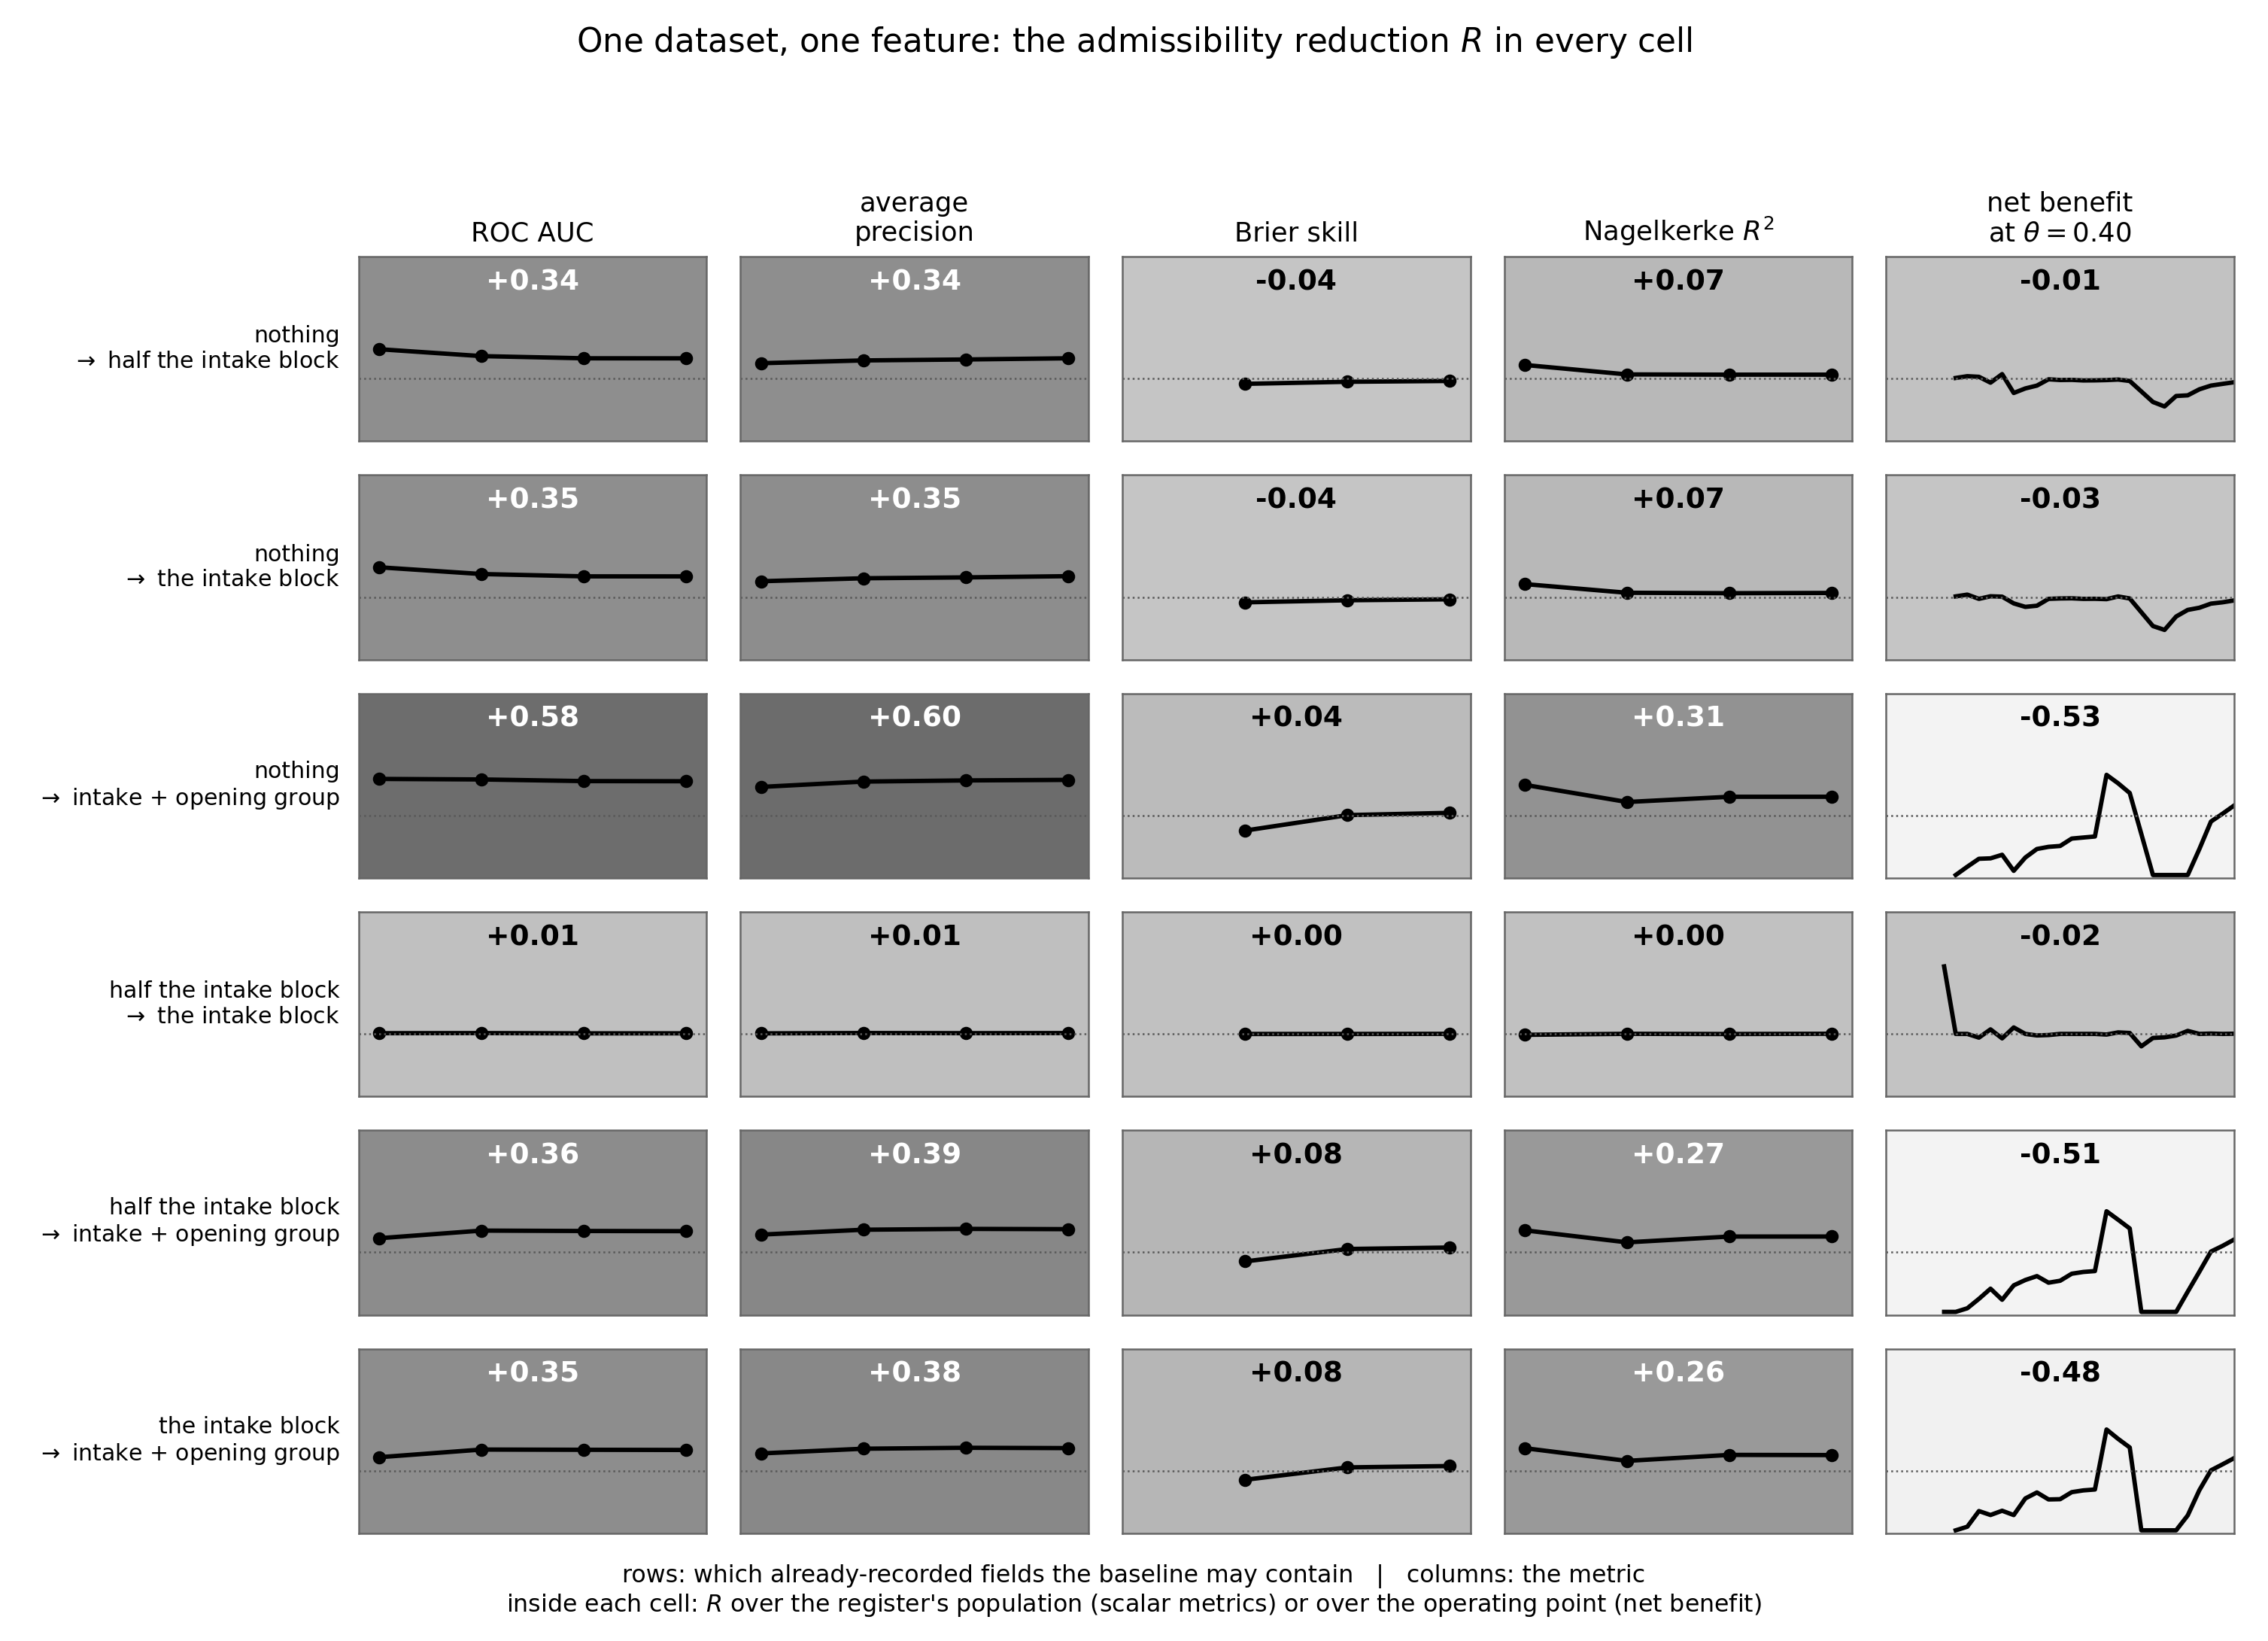
\includegraphics[width=\linewidth]{fig_signature.png}
\caption{The same data, the same feature, and every defensible answer at once. Each cell is the admissibility reduction $R$ for item identity on BPI Challenge 2014: rows are which already-recorded fields the baseline is allowed to contain, columns are the metric, and the curve inside a cell runs over the register's population (scalar metrics) or over the operating point (net benefit). The reference values printed in the cells run -0.53 to +0.60. WHAT THIS FIGURE DOES NOT SHOW: it carries no intervals --- every cell is a point estimate, and the bootstrap intervals are in Table~\ref{tab:instruments} and in \texttt{results/r44\_spread.csv}; it shows one log, and the same grid for two further organisations is in the same file; and it shows the reduction, not the increment, so a cell where the entity is worth almost nothing to begin with looks the same as one where it is worth a great deal. The in-cell curves are clipped to $[-1,2]$ and the unclipped values are in \texttt{results/r47\_cells.csv}.}
\label{fig:signature}
\end{figure}

\paragraph{Is this one paper or three?}
An editor is entitled to ask, because a literature audit, a set of
propositions with a simulation, and an empirical study of a configuration
database are three literatures. They are one paper here for one reason:
\textbf{each of the three is the answer to an objection the other two
provoke, and separately each is refutable in a way the three together are
not.} The empirical study alone is a null on one estate, and the obvious reply
is that the choices behind it were made badly. The propositions alone say what
can happen and nothing about what does. The audit alone measures a reporting
practice without showing that the practice costs anything. Together they say:
here is what the field does, here is what can happen in principle, and here is
what does happen on real data when you vary the choices the field does not
vary --- and the third of those is the one axis on which the audit finds
\emph{zero} papers. Split the paper and each piece loses its own defence. We
say this here rather than in a cover letter because a reader is entitled to
the reason at the point they first wonder.

\paragraph{What kind of contribution this is.}
We report no deployed system. This is a retrospective study on two public
benchmarks, offered as an evaluation practice.
Section~\ref{sec:buys} states what the choice costs in units closer to those
a service desk operates in, and Section~\ref{sec:layer} states which
\emph{layer} of configuration data carries the value, which is the question a
buyer actually faces.

\section{Background}
\label{sec:background}

\paragraph{Prediction on incident event logs.}
Our task sits at the boundary of predictive process monitoring, surveyed and
benchmarked across real-world logs \citep{teinemaa2019outcome,verenich2019survey}
on data of the kind process mining formalises \citep{vanderaalst2016process}.
We predict at $t=0$ from creation-time attributes with no prefix, which is
tabular classification on a process log rather than prefix-based monitoring
in the sense those benchmarks evaluate; we note that
\citet{teinemaa2019outcome} explicitly excluded the 2013 and 2014 BPI
Challenge logs from their benchmark for lacking a static/dynamic attribute
split. The BPI Challenge logs are the standard public instances
\citep{vandongen2014bpic,steeman2013bpic}; comparable exports exist elsewhere
\citep{amaral2018incident}. Such logs carry documented quality hazards
\citep{suriadi2017imperfection}. One hazard bears directly on us and we
state it as our own measurement rather than attributing it: values recorded
once per record can be replicated onto every event of that record, which
makes constancy across a case uninformative about when the value became
known. Establishing what a resource stamp on an event denotes is the business
of organisational mining \citep{vanderaalst2005social}, which is what
Section~\ref{sec:data} does from first principles for the field our result
turns on. The state of the queue a case arrives into --- the inter-case
perspective --- carries real predictive content in this setting
\citep{senderovich2017intercase}, and Section~\ref{sec:admission} admits four
free creation-time congestion features to the baseline for that reason.

\paragraph{The CMDB and what justifies it.}
A CMDB records configuration items and their relationships, and is the asset
on which the configuration-management practice of ITIL and its successors
rests. Survey work on ITSM framework adoption \citep{marrone2011itil} finds
that realised benefits grow with implementation maturity, but measures them
as practitioner-reported outcomes rather than as the analytic value of the
configuration data itself.

\paragraph{What is and is not already measured.}
Prior peer-reviewed work uses the affected configuration item as one input
among many without isolating its value. \citet{schad2022reassign} predict
ticket reassignment --- our own target --- with a relational graph
convolutional network on a public ServiceNow log, with the configuration
item among the incident-node features. \citet{sarnovsky2018predictive}, working
on the same Rabobank log we use, report ROC AUC and rank CI type, CI subtype
and service component among the most significant attributes.
\citet{kapel2026change} predict change-induced incidents at a large bank and
rank CI Name third by SHAP importance, behind two free-text fields. None of
the three performs a controlled with-and-without comparison attributing a
change in a fixed metric to configuration-item identity against a stated
baseline, which is what we do; but the reader should note that the
question is not untouched, and that in the one study which ranks a
free-text field against the configuration item, free text wins.

\paragraph{The methods a CMDB is bought to enable.}
Surveys of AIOps for failure management
\citep{zhang2024aiops,remil2024aiops,notaro2021aiops} catalogue triage,
failure-prediction and root-cause methods that take configuration data as
input. Incident triage in particular --- deciding which team owns an
incident --- has been treated as a learning problem on operational logs at
industrial scale \citep{chen2019triage}, as has failure prediction across a
cloud estate \citep{lin2018node}.

\paragraph{What the comparison is measured against.}
The value of a feature \emph{given} a baseline is what algorithm-agnostic
variable-importance frameworks formalise; \citet{williamson2021vimp} develop
this for $R^2$-type predictiveness and \citet{williamson2023vimp} extend it
to AUC, which is our metric. Our overlap is the redundancy that additive
importance measures share credit for \citep{covert2020sage}.
Section~\ref{sec:notvimp} says what this paper adds to those frameworks and
what it does not.

The estimand itself --- the change in a fixed metric when one variable joins
an existing model --- has been argued over in biostatistics for two decades,
and that literature reached our conclusion first. \citet{cook2007roc} shows
that an increment in AUC is a poor measure of a variable's incremental value
and depends heavily on the model it is added to. \citet{vickers2006dca}
supply the principled replacement for the capacity-limited framing we used in
earlier versions and withdraw in Section~\ref{sec:buys}. We claim no priority
over these; we report that the failure mode they describe is, on operational
data, large enough to change a procurement decision.

Within machine learning, \citet{rendle2019baselines} and
\citet{dacrema2019progress} show insufficiently tuned baselines accounting for
reported gains in recommender systems; benchmark conclusions are sensitive to
variation that is seldom reported \citep{bouthillier2021variance}, and
documentation of the choices producing a result is thin
\citep{gundersen2018reproducibility}. Where the choice concerns which fields
may enter, it shades into leakage \citep{kaufman2012leakage,kapoor2023leakage},
whose formal treatments accommodate admission rules as constraints set by the
problem definition rather than derived from it. In predictive process
monitoring, \citet{weytjens2022leakage} show that avoiding a different
leak --- case prefixes shared between training and test under naive temporal
splitting --- needs explicit construction; we adopt their strict temporal
splitting and, at their prompting, examine the extract boundary in
Section~\ref{sec:data}. We report a field-admission failure mode for a
deployment decision rather than a leaderboard, where it is not a modelling
detail but the number the business case turns on.

\section{This Is Not Just Conditional Variable Importance}
\label{sec:notvimp}

\subsection{The estimand}
Equation~\ref{eq:estimand} names
$V(f \mid B, m, \theta) = m(B \cup \{f\}, \theta) - m(B, \theta)$. For two
nested baselines $B_0 \subset B_1$ we report the \emph{admissibility
reduction}
\begin{equation}
R(f \mid B_0, B_1, m, \theta) \;=\; 1 - \frac{V(f \mid B_1, m, \theta)}
{V(f \mid B_0, m, \theta)},
\label{eq:reduction}
\end{equation}
the share of a feature's apparent value already carried by fields the
organisation records for nothing. $\theta$ is absent for metrics that
integrate over the operating range; Section~\ref{sec:metric} says which those
are. We report $R$ only where $V(f \mid B_0, m, \theta)$ is positive in every
bootstrap draw. A ratio whose denominator crosses zero is not a quantity, and
this paper has previously printed one that did.

Three properties of $R$ should be stated before it is used, because each is a
limit a reader would otherwise have to infer.

First, $R$ is metric-relative \emph{by construction}. It divides two
increments of $m$, and an increment of AUC has no natural zero of the kind a
ratio needs, so ``$43.7\%$ of the value is absorbed'' under AUC and
``$60.3\%$'' under average precision are not one quantity measured twice. We do not
claim $R$ is comparable across $m$; Section~\ref{sec:metric} reports the
spread across $m$ as the finding.

Second, every interval in this paper comes from a paired bootstrap that
resamples test rows and holds the fitted models fixed. It therefore quantifies
test-set sampling error and not model-fitting variability, and is narrower
than a full resampling would give. The substitute is the design-space sweep
this paper already carries --- split point, target threshold, cleaning cutoff
and three estimator families --- across which the AUC reduction runs $36.1\%$
to $48.3\%$. A reader should treat that range, not a bootstrap interval, as
the honest width.

Third, four is a claim about how many choices are usually left \emph{implicit},
not about how many exist. The estimator family is a fifth and the cohort a
sixth; the literature already treats the estimator as a choice, and this paper
varies it over three families and reports the range. The four below are the
ones a feature-value claim routinely fixes without saying so.

Four independent choices therefore sit inside any single-number claim: which
already-recorded fields $B$ contains, which $m$, which $\theta$, and --- for a
feature that is a lookup into a register --- how completely that register is
populated. Sections~\ref{sec:admission}, \ref{sec:metric}, \ref{sec:opp}
and~\ref{sec:population} vary one at a time on one dataset, holding the cohort,
the split, the estimator and the seed fixed throughout, so that any movement
is attributable to the choice and to nothing else.
Section~\ref{sec:standard} states what we propose be reported in place of a
point.

\subsection{What is and is not new here}
The objection we expect first is that measured importance is baseline-relative,
that \citet{williamson2023vimp} and \citet{covert2020sage} formalise exactly
that, and that a study reporting it on one log is reporting a known fact with
a new number attached. The objection is correct about the formal content and
we concede it in those terms. Four things are added here that no formal
framework supplies.

\paragraph{A magnitude on a named decision.}
Those frameworks establish that a feature's importance is defined only
relative to a baseline. They do not say how large the dependence is for any
particular feature on any particular decision, and a procurement decision
turns on the size. On this task the answer is that the choice of baseline
moves the measured value of an entire data programme by roughly half, and
that half is the difference between an investment case and none.

\paragraph{The right estimand is not an average over baselines.}
A Shapley-style attribution averages a feature's contribution over subsets of
the others, which is the correct thing to compute when the question is how to
apportion credit within a fixed model. It is the wrong thing to compute here.
A business case needs a feature's value against \emph{the baseline the
organisation will actually have} --- the fields already in its ticketing
tool --- not an average over baselines it will never be in. We therefore
report a ladder over named, admissible baselines rather than a single
attribution, and Section~\ref{sec:data} states the admissibility criterion
before applying it.

\paragraph{The overlapping field is free.}
The interesting case is not that some baseline choice changes the answer; any
correlated feature does that. It is that the field which absorbs half the
measured value is one the organisation \emph{already records at no cost},
sitting in the same export, requiring no programme and no budget line. That
is what makes the analyst's choice invisible rather than merely arbitrary:
nothing in the data flags the omission, and the omitted field has no price
tag to prompt a question about it.

\paragraph{The metric argument is not in those frameworks at all.}
\citet{williamson2023vimp} and \citet{covert2020sage} are stated for a fixed
predictiveness measure. Nothing in them says that two defensible measures
applied to the \emph{same scores} disagree about how much of a feature's value
a second feature absorbs, still less by how much. That is an empirical
question, Section~\ref{sec:metric} answers it here, and the answer is that on
this decision the metric choice moves the reduction by more than the free
field does.

\paragraph{Where it appears and where it does not, measured rather than
assumed.}
Baseline-relativity is a theorem; whether a particular pair of fields overlaps
in a particular estate is an empirical question with no general answer. We
pre-registered a protocol and applied it to $22$ public logs
(Section~\ref{sec:corpus}) rather than generalising from one. The answer is
mostly negative and is reported as such.

\paragraph{What we do not claim.}
We do not claim a new estimator, a new importance measure, or priority over
\citet{cook2007roc}, who stated the underlying point for AUC in 2007. Nor do
we claim any of the four choices is illegitimate: each is correct about the
question it asks. The contribution is that those are different questions,
that a single number answers one of them without saying which, and that on
this decision the spread between them is larger than the effect.

\subsection{Three propositions about what can and cannot happen}
\label{sec:props}

That $V$ depends on its arguments is a theorem and not ours. What is not in
the frameworks above is \emph{how far} the dependence can go, \emph{which}
instruments can see \emph{which} choice, and whether knowing the effect of one
choice constrains the effect of another. Three small results, each with a
constructive proof that a reader can execute
(\texttt{scripts/r41\_propositions.py}; the constructions are in
Appendix~\ref{app:props}). They are small and we say so: their job is to move
this paper's contribution from ``measured some magnitudes'' to ``established
what can and cannot happen, and then measured what does''.

\paragraph{Proposition 1 (metric-unboundedness).} For a target
$r \in [0,1)$ there exist score distributions, a baseline $B_0$, a feature $f$
and two defensible metrics under which the admissibility reduction $R$ equals
$r$ and $0$ respectively.

\emph{Construction.} Let every model's score take one of two values, so each
is described by the counts $(a,b)$ of positives and negatives in the high
block. With $P$ positives, $N = \rho P$ negatives, $\alpha = a/P$,
$\beta = b/N$ and $\pi = 1/(1+\rho)$, two identities hold exactly:
$\mathrm{AUC} - \tfrac12 = (\alpha - \beta)/2$, and
$\mathrm{AP} - \pi = \alpha\left(\alpha/(\alpha + \beta\rho) - \pi\right)$.
Take both baselines to be the fully tied model. Fixing $\alpha - \beta = d$ on
both legs makes the AUC increments identical, so $R$ under AUC is
\emph{exactly} zero; sliding $\alpha$ along $[d,1]$ moves the AP increment
monotonically. Executed over ten targets, $R$ under ROC AUC is zero to
$4.4 \times 10^{-16}$ --- floating-point noise, not approximation --- while
$R$ under average precision hits every target from $0.05$ to $0.99$ to within
$1.8 \times 10^{-4}$, \textbf{on identical scores}. The declared family
reaches $0.998$; that bound is reported rather than assumed away, and it
widens with $\rho$.

This is the analytic form of what Section~\ref{sec:metric} measures: $43.7\%$
under AUC against $60.3\%$ under average precision, on scores that do not
move.

\paragraph{Proposition 2 (the rank-invariance boundary).} $R$ is invariant
under every strictly increasing transformation of a model's scores
\textbf{if and only if} the metric is rank-based.

\emph{Proof.} ($\Leftarrow$) A strictly increasing $\varphi$ preserves the
weak ordering, so a rank-based $m$ is unchanged, so every $V$ is unchanged,
so $R$ is. ($\Rightarrow$) If $m$ is not rank-based there are $s, s'$ inducing
the same weak ordering with $m(s) \neq m(s')$; equality of the weak ordering
makes $s_i \mapsto s'_i$ well defined and strictly increasing on the distinct
values of $s$, and any such map extends to a strictly increasing $\varphi$ on the
real line. Applying it to one leg changes that leg's $V$ and hence $R$.
\hfill (QED)

\emph{Witness.} On a synthetic ladder, applying one strictly increasing
$\varphi$ to the naive leg's scores moves $R$ by exactly $0.000000$ under ROC
AUC and average precision and by between $1.645$ and $4.255$ under Brier
skill, Nagelkerke $R^2$ and net benefit at two operating points.

The proposition converts Section~\ref{sec:metric}'s recalibration result from
an observation into a statement about \emph{which instruments can see
calibration at all}: recalibrating the models moves the proper-score
reductions and leaves the rank-based ones at exactly zero, and no
implementation detail can change that.

\paragraph{Proposition 3 (non-redundancy).} No one of the four choices
determines another: for an ordered pair of axes $(X,Y)$ there exist two
configurations agreeing on how much $X$ moves the answer and differing on how
much $Y$ does.

\emph{Construction, and its limit.} Over a declared family of $18$ synthetic
estates --- varying how tightly the opening field is coupled to the entity,
how much of the entity's signal it carries, and how strong the entity is ---
we search all twelve ordered pairs. \textbf{Ten of the twelve are
constructible} at the declared tolerances. The two that are not are
$(\text{metric}, \text{threshold})$ and $(\text{population},
\text{threshold})$, and the reason is stated rather than hidden: the
threshold axis's spread across this family is an order of magnitude larger
than the others, so the ``differ by a quarter of the axis's own range''
criterion demands a gap of
$3.396$ and the best pairs found reach $1.907$ and $2.913$. That is a
property of the tolerance and of the threshold axis's scale, not evidence
that those pairs are redundant, and we report the two failures rather than
retuning until twelve appear.

\textbf{How much the count depends on that tolerance is itself measured},
because a referee is entitled to ask and the answer is not flattering to a
single reported figure: across a grid of $16$ tolerance pairs the number of
constructible axis pairs runs from $8$ to $12$. The paper reports the cell at
(agree within $5\%$ of the axis's range, differ by $25\%$ of it); the whole
grid is in \texttt{results/r49\_prop3\_tol.csv}.

\section{How the Field Reports Feature Value Today}
\label{sec:audit}

Everything above is an argument that four choices set the answer. A referee is
entitled to reply that the argument is a known critique --- Cook on AUC
increments, Hand on metric incoherence, Vickers and Elkin on operating points,
Williamson and Covert on baseline-relativity --- and that a critique everybody
already accepts needs no paper. The reply to that is a measurement: a critique
everybody accepts and nobody follows is not a known critique but a documented
practice failure, and this section documents one.

\subsection{What was registered, and when}
\label{sec:audit:reg}

\texttt{AUDIT-PROTOCOL.md} fixes the frame, the retrieval rule, the inclusion
rule, five codes and the reliability design. It was committed \emph{before a
single paper was screened}, in a commit that adds no
\texttt{results/r40\_*.csv} and no downloaded full text; \texttt{git log
--stat} shows it arriving alone. Section~1 of that document states, in
advance, the outcome that would refute this paper's premise: a majority of
included papers stating their baseline \emph{and} a majority justifying their
metric. That outcome did not arrive, but something close enough to it did that
the paper's wording had to change, and \S\ref{sec:audit:verdict} says so.

\paragraph{The frame.} Two frames, unioned and deduplicated on DOI, enumerated
through the OpenAlex API so that a reader can re-run the query rather than
trust a description of it. \emph{Frame A}: research articles published
$2019$--$2026$, open access, in \emph{Information Systems}, \emph{Decision
Support Systems}, \emph{Information \& Management} and \emph{Empirical
Software Engineering}, passing a declared topical pre-filter on title and
abstract. \emph{Frame B}: every open-access work $2019$--$2026$ citing either
OpenAlex record of Teinemaa et al.'s outcome-oriented predictive process
monitoring benchmark~\citep{teinemaa2019outcome}.

\paragraph{The conference venues, and why they are not in the frame.} The plan
this round executed named BPM, ICPM and CAiSE. They are not machine-enumerable
in OpenAlex and we do not pretend otherwise: measured on 2026-08-22, before any
screening, the BPM source record carries $69$ works for $2019$--$2026$ and
\emph{none} flagged open access, the CAiSE record carries one, and a search
for ICPM returns an unrelated serial. Most papers from those venues are
indexed under the umbrella LNCS source, which cannot be filtered to a
conference. A frame that cannot be reproduced is not a frame. Those venues
are covered through Frame~B instead, and the venue mix of the included set is
reported below whatever it turns out to be.

\subsection{The funnel}
\label{sec:audit:funnel}

The two frames yield $607$ works, $604$ after deduplication, and the
registered cap of $600$ is applied by simple random sample with seed
$20260819$. Full text is retrieved for $369$ of the $600$ --- $61.5\%$ --- and
this is the stage that loses the most, for reasons nobody can show are related
to the codes and which \S\ref{sec:limits} declines to assume away. Of the
$369$, $192$ report no quantitative performance metric and $123$ carry no
comparison of performance with and without a named feature. \textbf{The
included set is $54$ papers across $15$ venues.}

The screening rule is a pattern set fixed in \texttt{r40\_audit.py} before the
first paper was read, and every included paper's record carries the sentence
that admitted it, so the inclusion decision is as auditable as the codes.
Reading the first run's output found three patterns that did not implement the
rule written above them --- the ``with\slash without'' class admitted
``Without basic knowledge over the data domain'', and three of the five codes
matched sentences about something other than the model's evaluation.
Amendment~1 to the protocol records all three, and \emph{both} codings are
reported: the registered screen admits $117$ papers, the amended screen $54$,
and \texttt{results/r40\_proportions.csv} carries the proportions under each.

\subsection{The codes, and what a mechanical coder is worth}
\label{sec:audit:codes}

Five binary items per included paper, each with a mechanical rule, each
carrying a verbatim quote and the PDF page it was found on:
\texttt{B\_stated} (is the baseline's feature set enumerable from the paper?),
\texttt{B\_justified} (is the exclusion of an already-available field
argued?), \texttt{M\_justified} (is the metric argued for, not merely named?),
\texttt{Theta\_stated} (is an operating point or a cost ratio stated, or is
the metric explicitly said to integrate over them?), and
\texttt{Range\_reported} (is the \emph{increment} reported at more than one
level of any of the four choices?).

\textbf{A mechanical coder is not a reader, and this paper's primary numbers
are not the mechanical ones.} Thirty included papers were drawn with the
registered seed and coded by reading a deterministic extract of each --- every
sentence carrying a metric and a number, and every sentence carrying baseline,
feature, threshold, cost or metric-justification vocabulary --- written to
\texttt{data/audit/adjudication/} so that the evidence a code was assigned
from is as public as the code. Two things came out of that reading and both
are reported rather than repaired.

First, \textbf{the screen's precision is $66.7\%$}: of the thirty papers the
amended screen admitted, a read confirms $20$ as reporting a quantitative
comparison of predictive performance with and without a named feature. The
other ten compare a resampling technique, a preprocessing pipeline, a set of
method components or, in one case, human reading behaviour.

Second, \textbf{the mechanical coder under-detects badly}. Against the read it
missed $39$ \texttt{yes} codes and asserted $9$ a read does not support; on
\texttt{Range\_reported} it found none where a read finds $11$ of $20$. The
mechanical proportions are therefore reported as a \emph{lower bound}, in
those words, and the adjudicated proportions on $n=20$ are what
Table~\ref{tab:audit} prints first.

\begin{table}[htbp]
\centering
\caption{How the field reports the incremental value of a field. Adjudicated
by reading, on the $20$ papers a read confirms are in scope; the mechanical
coder's proportions on all $54$ included papers are printed beside them and
are a lower bound, not an estimate. Intervals are Wilson binomial $95\%$.}
\label{tab:audit}
\begin{tabular}{lrlrl}
\toprule
& \multicolumn{2}{c}{adjudicated, $n=20$} & \multicolumn{2}{c}{mechanical, $n=54$} \\
\cmidrule(lr){2-3}\cmidrule(lr){4-5}
code & yes & share & yes & share \\
\midrule
\texttt{B\_stated}       & $8$  & $40.0\%$ $[21.8,61.4]$ & $4$  & $7.4\%$ $[2.9,17.6]$ \\
\texttt{B\_justified}    & $5$  & $25.0\%$ $[11.1,46.9]$ & $6$  & $11.1\%$ $[5.1,22.2]$ \\
\texttt{M\_justified}    & $10$ & $50.0\%$ $[29.9,70.1]$ & $10$ & $18.5\%$ $[10.3,30.9]$ \\
\texttt{Theta\_stated}   & $12$ & $60.0\%$ $[38.6,78.2]$ & $14$ & $25.9\%$ $[16.1,39.0]$ \\
\texttt{Range\_reported} & $11$ & $55.0\%$ $[34.2,74.2]$ & $0$  & $0.0\%$ $[0.0,6.7]$ \\
\bottomrule
\end{tabular}
\end{table}

\subsection{The result, and what it does to this paper's premise}
\label{sec:audit:verdict}

\paragraph{The strong claim is false and comes out.} We expected to find that
a large majority of papers state none of the four choices. They do not. Two of
five enumerate their baseline, half argue their metric, and three in five
state an operating point or say explicitly that their metric integrates over
one. A field that does that is not ignoring the critique.

\paragraph{What survives is narrower and, we think, sharper.} Reporting the
increment at more than one level of \emph{some} choice is common. It is almost
never more than one choice, and it is almost always the same two.

\emph{What counts as a range here is stated before the numbers, because the
rule is generous and the generosity works against this paper.} A paper is
credited with reporting a range over the metric if it reports the
with-and-without difference under two or more metrics --- ordinary practice,
and a long way from the surface this paper argues for. Crediting it is
deliberate: a stricter reading would make the field look worse against a
standard nobody has adopted. On the two axes where the count is zero, no
softer reading was available to give.

\begin{itemize}
\item over the \textbf{metric}: $9$ of $20$, $45.0\%$ $[25.8,65.8]$;
\item over the \textbf{baseline}: $6$ of $20$, $30.0\%$ $[14.5,51.9]$;
\item over the \textbf{operating point}: $\mathbf{0}$ \textbf{of} $\mathbf{20}$, $0.0\%$ $[0.0,16.2]$;
\item over the \textbf{register's population}: $\mathbf{0}$ \textbf{of} $\mathbf{20}$, $0.0\%$ $[0.0,16.2]$;
\item over \textbf{two or more} of the four at once: $4$ of $20$, $20.0\%$ $[8.0,41.7]$.
\end{itemize}

Not one paper in the subsample reports what a feature is worth across a range
of operating points, and not one across a range of register populations.
Those are exactly the two axes on which this paper's own headline moves most:
Section~\ref{sec:opp} puts the reduction between $4.7\%$ and $134.1\%$ across
the operating range, and Section~\ref{sec:population} moves it by a quarter of
its own size across the population curve. The practice failure this paper
documents is not that the field ignores its own critiques. It is that the
field varies the two choices that are cheap to vary and does not vary the two
that decide the answer.

\paragraph{The topical pre-filter is a constructed control, so it is
nulled.} Frame A applies a declared keyword filter to titles and abstracts;
frame B applies none. If the filter selected papers that happen to be more
careful about their evaluation, the audit would \emph{understate} the practice
failure --- and it does. On the four codes where the two frames can be
compared, the filtered frame's papers are more careful on every one, by up to
$23.3$ percentage points on \texttt{M\_justified}. On
\texttt{Range\_reported} both frames are at zero. The unfiltered arm is only
$11$ papers, so this is a direction and not an estimate; the direction is the
conservative one, and \texttt{results/r49\_frame\_null.csv} carries all five
codes.

\paragraph{Reliability, with one author.} A single author coded every paper,
by machine, and then read thirty. That is not inter-rater reliability and this
paper does not call it that. What is reported instead: every code ships with
its quote and page, so the coding is auditable rather than trusted; a second,
independently written implementation of the same five rules agrees with the
first on a random $20\%$ of the included set with Cohen's $\kappa$ between
$0.256$ and $0.501$, which is \emph{poor}, and is printed here because it is
the honest measure of how much the operationalisation matters; and the
seven-day blind re-code by the author is written into
\texttt{submission/OWNER-ACTIONS.md} with the sample already drawn, because it
needs elapsed time and a human, and an agent has neither.

\subsection{What this costs a reader, worked on a public dataset}
\label{sec:audit:worked}

The consequence is easiest to see away from event logs. UCI Adult
(\texttt{doi:10.24432/C5XW20}) predicts whether income exceeds \$50k. Suppose
an analyst reports what \texttt{occupation} is worth: it is the expensive
field, the one a survey has to ask about and code, where age, sex, race and
country come free with the sampling frame and education comes with the
enrolment record. Running the surface with the package this paper ships:

\begin{itemize}
\item against the fields that come free with the frame, admitting
\texttt{occupation} on top of them absorbs $R = +0.749$ of what it looked
worth against nothing;
\item against those plus education and hours worked, $R = +0.200$.
\end{itemize}

Same data, same feature, same metric, same operating point. \textbf{The
baseline alone moves the answer by three quarters of its own size.} We name no
defect in any paper in doing this, and the point is not that anyone was
careless: the practice is universal, this paper's own earlier versions
included, and Section~\ref{sec:corrections} is the evidence for that.

\section{Data and Task}
\label{sec:data}

\subsection{The primary organisation}

We use the incident records of the BPI Challenge 2014 log
\citep{vandongen2014bpic} from Rabobank Group ICT, recorded in HP Service
Manager, with the activity log shipped alongside. The configuration-item
column we use is \texttt{CI Name (aff)}, the item affected at the time the
incident was recorded, not the closure-time \texttt{CI Name (CBy)}.

\paragraph{Cleaning.}
Of $46{,}809$ rows, $203$ carry no incident identifier and one an unparseable
timestamp. A further $1{,}150$ opened before 2013-10-01 are left-censored ---
already open when the extract began --- and are reassigned at $81.2\%$
against $40.0\%$ for the incidents we keep. Removing them leaves
$\mathbf{45{,}455}$ incidents to 2014-03-31; a temporal $70/30$ split gives
$31{,}818$ training and $13{,}637$ test, positive rates $0.413$ and $0.372$.
The cutoff is not taken from the outcome: monthly volume rises from $857$
incidents in September 2013 to $8{,}606$ in October. The extract is
right-censored too --- incidents opened near its end cannot have long lives
--- so we re-measured on cohorts truncated up to a month early; the shrinkage
moves between $42\%$ and $45\%$, so the boundary does not drive it. The
affected-item field is $100\%$ populated across $2{,}929$ items, $2{,}554$
seen in training. That population rate is a property of the extract and of a
tool configuration that copies the item onto the incident from the
originating interaction record; it is not evidence about CMDB accuracy in
general, and Section~\ref{sec:limits} returns to the point.

\paragraph{Task and estimator.}
Predict at creation whether an incident will later be reassigned. We call
the target reassignment rather than misrouting throughout: it fires on
$37.2\%$ of test incidents, which is routine handling and not error, and
Section~\ref{sec:buys} reports the ladder at stricter thresholds. Median
handling time rises from $1.59$ hours for incidents never reassigned to
$47.53$ hours for those reassigned five or more times; we use this to
motivate the task, not as a recoverable saving.

The intake block is four fields carried on the incident form: Category,
Impact, Urgency and Priority. It is effectively three. \texttt{Priority} is a
deterministic function of \texttt{(Impact, Urgency)} on this log --- $19$
occupied cells, none carrying more than one Priority, across all $46{,}809$
rows --- so it adds no information, and dropping it moves intake AUC from
$0.562$ to $0.564$. \citet{sarnovsky2018predictive} reported this redundancy
on this same log in 2018. We keep the column because it is what an analyst
building the naive arm would include, and we disclose it because a paper
arguing that baselines are under-specified should not ship an
under-specified baseline in silence. The four fields together take only $23$
distinct combinations in training and $23$ in test, which is a fact
Section~\ref{sec:buys} needs and which no choice of estimator can change.

The primary estimator is one-hot logistic regression, chosen because it is
bin-free: scikit-learn's \texttt{LogisticRegression} with L2 penalty,
inverse regularisation strength $C=1.0$, the \texttt{lbfgs} solver and a cap
of $3000$ iterations, with \texttt{OneHotEncoder} set to ignore unseen
levels. The penalty is held fixed across every arm; tuning it per arm on an
inner split of training data moves the headline reduction from $43.7\%$ to
$43.2\%$. Two further estimator specifications are reported in
Section~\ref{sec:admission}. Encoders and rankings are fit on training data
only; intervals are $2{,}000$-resample paired bootstraps, except
Table~\ref{tab:tie}, whose counts are re-ranked in each draw and use
$400$. Monte-Carlo nulls use $15$ to $100$ draws, the count set by cost and
recorded in the code that produces each. Every sampling script is seeded
from a single constant, so the reported figures are reproducible exactly.

\paragraph{The free field, and what it is not.}
The activity log records, on the \texttt{Open} event of every incident, an
assignment group: $49$ in training, none missing. An earlier draft of this
paper called it the queue the service desk routed the incident to. That was
an assertion, not a finding, and it is wrong. Three checks say so. The
\texttt{Open} rows carry $50$ distinct groups where the \texttt{Assignment}
rows carry $218$, and a routing destination cannot be less diverse than the
teams that then do the work. One group accounts for $67.0\%$ of
\texttt{Open} rows but only $18.4\%$ of all activity rows. And the
\texttt{Open} group matches the group on the incident's first
\texttt{Assignment} activity for just $15.1\%$ of the $37{,}577$ incidents
that have one. The field is the group that \emph{logged} the incident: one central desk for
two thirds of tickets, a long tail for the rest. We do not characterise that
tail --- its openers match the first \texttt{Assignment} group only $21.8\%$
of the time and appear anywhere in the later work rows only $59.1\%$, so
calling them teams opening their own work would be another assertion of the
kind we are correcting.
It is also concentrated and unstable: the largest group holds $62.1\%$ of
training incidents, and the number of live groups falls from $49$ to $32$
between our two halves, while in the test half it logs $78.6\%$ of
incidents.

\paragraph{The free field is not a restatement of the target.}
A reader may reasonably suspect the opposite of what
Section~\ref{sec:mechanism} argues: that a field naming a \emph{group}
cannot help but encode a target defined as a \emph{change of group}, making
the whole ladder circular. That reading makes a directional prediction, and
the data contradicts it. The central desk logs most tickets and does a small
minority of the work, so on the circular reading it should be the one handing
work on, and should reassign more than everyone else. It reassigns
\emph{less}: $0.309$ against $0.603$, a difference of $-0.294$
$[-0.315,-0.275]$. What the field separates is a low-reassignment intake
channel from a high-reassignment one. Nor is it a strong predictor in its own
right: the per-group outcome rate, applied as a lookup with no model, scores
$0.642$, and the one-bit central-desk contrast $0.606$. A field that restated
the target would score near the ceiling.

\paragraph{Why not the real routing decision.}
The obvious repair is not available. The first \texttt{Assignment} group
occurs strictly after \texttt{Open} on every incident that has one, a median
of $46$ minutes later, and $7{,}878$ of $45{,}455$ never have one. It fails
the criterion below, and substituting it would introduce the leakage that
criterion prevents.

\paragraph{Admissibility, and mutation.}
A field on the \texttt{Open} row is admitted only if it is a per-event
observation, tested by whether it varies across an incident's activity rows;
the opening group varies for $92.56\%$ of cohort incidents and matches the
last-observed group for only $21.35\%$. Because the incident file is a
closed-record snapshot we also report how often each field is edited after
creation: Urgency on $1{,}107$ incidents ($2.44\%$), Impact on $1{,}084$
($2.38\%$), the affected item on $159$ ($0.35\%$). Incidents whose Impact was edited are
reassigned at $0.66$ and those whose Urgency was edited at $0.67$, against
$0.39$ for the rest, so this is not neutral; Section~\ref{sec:admission} reports the headline with
those fields dropped and with the edited incidents removed. The activity log
carries no Category or Priority change type, so for those two fields the
snapshot cannot be audited at all; our disclosure covers the fields for which
an audit exists, not every field we use.

A second criterion governs the other direction, and Section~\ref{sec:layer}
needs it: a field may join the CMDB-free baseline only if the organisation
would hold it \emph{without} the CMDB. That excludes every field which is a
function of item identity, because such a field exists only where the item
register does.

\paragraph{The second organisation.}
A second public ITSM log, BPI Challenge 2013 incidents from Volvo IT Belgium, carries the same construction on a different estate and a different tool; its cohort, its target and what does and does not transfer are in Appendix~\ref{app:secondorg}, and its full surface is in Section~\ref{sec:threelogs}.

\section{The Admissibility Effect}
\label{sec:admission}

\begin{table}[t]
\centering\small\setlength{\tabcolsep}{6pt}
\begin{tabular}{@{}llccc@{}}
\toprule
Organisation & Baseline & AUC & +\,item id. & gain [95\% CI] \\
\midrule
Rabobank & intake only & 0.562 & 0.746 & $+0.183$ [$+0.172,+0.195$] \\
(BPIC 2014) & + opening group & 0.644 & 0.748 & $+0.103$ [$+0.094,+0.113$] \\
\midrule
Volvo IT & intake only & --- & --- & $+0.238$ \\
(BPIC 2013) & + opening group & --- & --- & $+0.092$ \\
\bottomrule
\end{tabular}
\caption{The value of knowing the affected configuration item, with and
without a field the organisation already records, on two organisations. The
Volvo rungs use a coarser item identifier and a more tightly coupled free
field; see Section~\ref{sec:secondorg}.}
\label{tab:headline}
\end{table}

\begin{figure}[t]
\centering
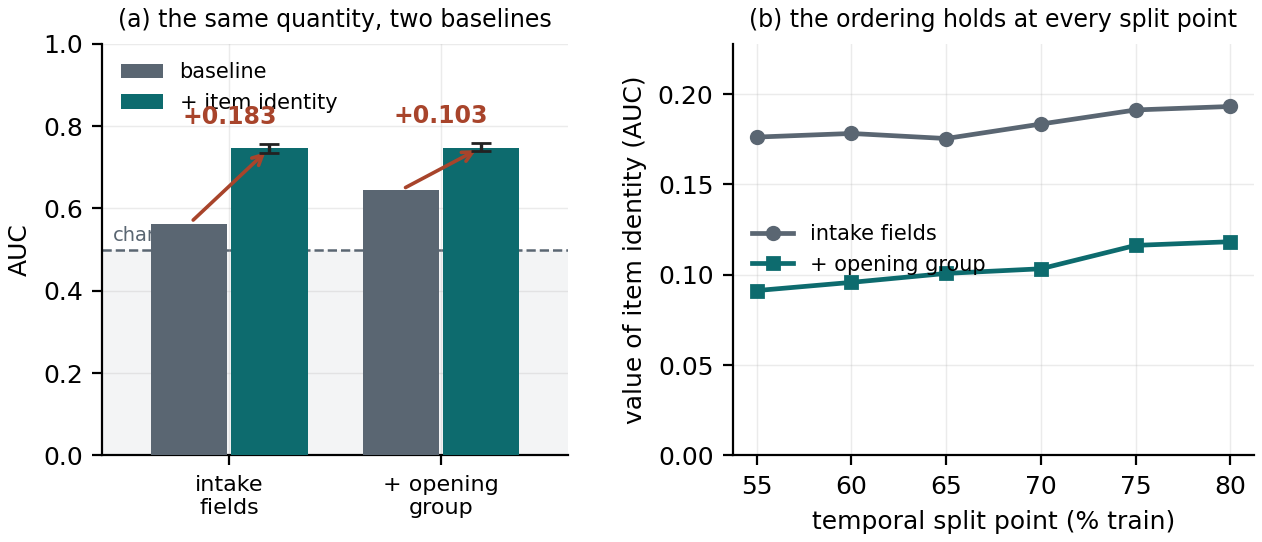
\includegraphics[width=\textwidth]{figJ1_baselines.png}
\caption{(a) The same quantity under two baselines, on the metric's full
range; the whisker on each treatment bar is the paired bootstrap interval of
that bar's own gain. (b) The ordering holds at every temporal split point
from $55\%$ to $80\%$.}
\label{fig:baselines}
\end{figure}

Against four intake fields the affected item looks decisive. Adding the
opening group cuts its measured value by $44\%$. The gains are roughly $28$ and
$17$ standard deviations outside a null in which the incident-to-item
association is shuffled, preserving column count and marginal distribution
while destroying the signal --- we round because re-drawing the same null at
a different draw count moves the first figure by about $0.7$ --- a comparison that matters because adding
item identity adds $2{,}554$ indicator columns, which is not free under a
fixed penalty. These $z$ figures pool the null's Monte-Carlo dispersion with
the gain's own bootstrap standard error; dividing by the null alone, as an
earlier draft did, would report $51$ and $33$. Because these nulls use as
few as $15$ draws, a two-digit $z$ is an extrapolation from a dispersion
estimate and not a tail probability; the load-bearing statement is that no
null draw comes near either gain.

It is not a split artifact: across six split points the two gains range
$+0.175$ to $+0.194$ and $+0.091$ to $+0.119$ (Figure~\ref{fig:baselines}b),
and across split point, target threshold and cleaning cutoff the second
ranges $+0.067$ to $+0.130$ --- wider than any bootstrap interval, which
conditions on all of those. Nor does the disclosed field editing explain it:
reducing the intake block to Category alone gives $+0.106$, and restricting
to the $44{,}227$ never-edited incidents gives $+0.107$.

\paragraph{The reduction, over the whole design space.}
The reduction rather than either gain is what we argue transfers, so it needs
the same disclosure. Across split points it runs $38.7\%$ to $48.3\%$; across
the three target thresholds $43.6\%$ to $48.3\%$; across the three estimator
specifications $42.7\%$ to $47.1\%$; and across five cleaning cutoffs from no
censoring removal at all to a two-month truncation, $36.1\%$ to $44.0\%$.
Over the whole design space it runs $\mathbf{36.1\%}$ to $\mathbf{48.3\%}$.
The bootstrap interval of $[40,48]$ we report at the published setting
conditions on every one of those knobs, and an earlier version of this paper
quoted it without saying so while asserting in its title that the reduction
was nearly a half. At the low end of the design space it is closer to a
third. What survives across the space is that the reduction is large and its
sign never changes.

\paragraph{It is not congestion.}
A reader from the process-mining community will ask whether the affected item
is standing in for load, since the inter-case perspective is known to carry
real content on this kind of log \citep{senderovich2017intercase} and neither
of our baselines looks at the state of the queue an incident arrives into.
Four features are free at creation and are computed from the open and close
timestamps of \emph{other} incidents, every one of which is in the past at the
moment of creation: the open backlog, arrivals in the preceding hour, hour of
day and day of week. Continuous features are cut at training deciles, so the
estimator is unchanged. Admitted to the baseline on the same criterion as the
opening group, they move the item's measured value from $+0.103$ to $+0.100$,
and the reduction from $43.7\%$ to $45.7\%$ $[41,50]$. Alone, without the
intake block or the group, the same four features score $0.497$ --- at this
horizon, on this log, creation-time congestion carries essentially nothing.
The item is not a load proxy.

\paragraph{It replicates on a second organisation.}
On Volvo IT the same ladder gives $+0.238$ against intake and $+0.092$ once
the opening group is admitted, a reduction of $61.3\%$ $[54,68]$; at the
stricter two-change threshold, $+0.249$ and $+0.139$, a reduction of $43.9\%$
$[31,55]$. Neither interval includes zero. Across six temporal split points
the first runs $60.3\%$ to $67.8\%$ and the second $40.8\%$ to $53.8\%$. The
qualitative claim --- that admitting one field the organisation already
records removes a large fraction of the item's measured value --- holds on a
second organisation, a second tool and a second country. The magnitude does
not transfer, and Section~\ref{sec:secondorg} gives a structural reason to
expect the Volvo figure to be the larger of the two.


\paragraph{It is not an artifact of the estimator.}
The dimensionality null rules out the regularisation burden of $2{,}554$
sparse columns, but a reader may want the effect shown where that burden
cannot arise. We re-represent item identity as a single cross-fitted
target-encoded column --- fitted on training only, out-of-fold, so no row
sees its own outcome --- which makes the item one continuous feature and
makes histogram boosting usable on a variable that otherwise collapses
$2{,}554$ items into $137$ bins. Across one-hot logistic regression,
logistic regression on the encoded item, and boosting on it, the first rung
ranges $+0.173$ to $+0.184$, the second $+0.091$ to $+0.104$, and the
reduction $42\%$ to $48\%$. Encoding a
\emph{shuffled} item column under the same pipeline returns
$-0.0001 \pm 0.0016$ and $+0.0042 \pm 0.0020$ on the group-aware rung. The
first collapses to zero; the second does not, and it is eleven standard
errors from zero, so it is a real systematic effect rather than noise and it
must be bounded on both rungs and not one. Run on the intake rung as well,
the same control returns $+0.0002 \pm 0.0015$ and $-0.0036 \pm 0.0025$.
Subtracting each rung's own residual from that rung's gain moves the
reduction from $42.7\%$ to $42.6\%$ under the encoded logistic model and from
$47.1\%$ to $50.5\%$ under boosting. The correction is therefore worth at
most $3.4$ percentage points and, where it bites, it makes the reduction
larger.

\paragraph{Three target definitions.}
Because reassignment is common, we repeat the ladder at stricter
thresholds. Requiring two or more reassignments ($21.8\%$ of incidents)
gives $+0.131$ and $+0.068$; three or more ($10.6\%$) gives $+0.151$ and
$+0.080$. The magnitude is threshold-dependent and not monotone, but the interval on
each $+$group rung excludes zero (we compute intervals for that rung only),
the ordering never reverses, and the reduction stays between $43\%$ and
$49\%$.

\paragraph{Does it survive a change of task?}
A gap on one target may be a property of it, so we repeated the ladder on two
further outcomes within the primary organisation. \emph{Reopening} is close
to an independent failure mode: $2{,}096$ incidents, correlating with
reassignment at $+0.14$. \emph{Long handling} --- handle time above the
training third quartile --- correlates at $+0.40$, so it is corroboration
only.

On reopening, item identity is worth $+0.083$ against the intake block and
$+0.055$ once the group is admitted, a reduction of $33\%$; on long handling,
$+0.118$ and $+0.078$, a reduction of $34\%$. Every rung sits outside its
matched-dimension null. But the reduction is what we argue transfers, so it
needs its own interval, and paired bootstraps give $[40,48]$ on reassignment,
$[28,38]$ on long handling and $[-1,60]$ on reopening. On the one target we
argue is near-independent the reduction is \emph{not} resolvably different
from zero ($P \le 0$ is $0.03$), and long handling, correlated at $+0.40$
with the primary target, cannot carry a replication alone. Reopening is rare
and its gains stand only $5.5$ and $4.2$ pooled standard deviations from
their nulls.

Cross-target replication within one organisation therefore fails to
resolve, while cross-organisation replication succeeds. We take the second
as the stronger evidence, because the objection it answers
--- that the effect is a property of one estate --- is the one a reader
should press hardest, and because both Volvo intervals exclude zero. The
reduction is largest on the target the opening group is most directly about,
which is consistent with Section~\ref{sec:mechanism} rather than predicted by
it: the mechanism says nothing about how the reduction should order across
targets.

\section{The Metric Axis}
\label{sec:metric}

Section~\ref{sec:admission} varied $B$ and held $m$ at ROC AUC. This section
holds $B$ and the scores fixed and varies $m$. Same cohort, same split, same
four fitted models, same seed: the only thing that changes is what is
computed from the scores.

\subsection{Seven instruments, six of them independent}
Table~\ref{tab:instruments} reports the reduction of Equation~\ref{eq:reduction}
under every instrument we can defend for this question. Detection at a fixed
review capacity is kept in the table although Section~\ref{sec:withdrawn}
withdrew it as a headline, because a matrix of instruments is the right place
to show what a tie-degenerate instrument does to a ratio.

Expected cost at a stated cost ratio is \emph{not} a seventh axis. At cost
ratio $r$ the Bayes threshold is $1/(1+r)$, so the net-benefit weight
$\theta/(1-\theta)$ is exactly $1/r$ and the cost avoided per case is
$r \cdot \text{NB}(1/(1+r))$ identically. The two therefore give the same
reduction; we verified it over ten contrasts, where the two agree to machine
precision, and report six instruments rather than seven.

\begin{table}[t]
\centering
\small
\begin{tabular}{lrrr}
\toprule
instrument & $V(f \mid B_0)$ & $V(f \mid B_1)$ & reduction \\
\midrule
ROC AUC              & $+0.183$ & $+0.103$ & $43.7\%$ $[40.1,47.1]$ \\
Average precision    & $+0.226$ & $+0.090$ & $60.3\%$ $[57.2,63.4]$ \\
Brier skill          & $+0.168$ & $+0.070$ & $58.4\%$ $[54.4,62.4]$ \\
Nagelkerke $R^2$     & $+0.223$ & $+0.097$ & $56.6\%$ $[52.8,60.3]$ \\
\midrule
Net benefit, $\theta=0.325$ & $+0.093$ & $+0.087$ & $6.3\%$ \\
Net benefit, $\theta=0.500$ & $+0.084$ & $-0.016$ & $119.2\%$ \\
\bottomrule
\end{tabular}
\caption{The same reduction under four instruments that integrate over the
operating range and two readings of one that does not. $B_0$ is the four
intake fields; $B_1$ adds the opening group. Intervals are paired bootstrap,
$2{,}000$ draws, one resampled index set per draw shared by all four models.
The net-benefit rows carry no interval on the ratio because the whole point of
the row pair is that the ratio is not one number.}
\label{tab:instruments}
\end{table}

\paragraph{The number we published is the smallest of them.}
Across the four instruments that integrate over the operating range the
reduction runs $43.7\%$ to $60.3\%$, and ROC AUC sits at the bottom of that
range. The previous version of this paper reported the AUC figure and treated
the more principled instruments as a threat to it; on this data they are not,
and a referee reading only Section~\ref{sec:withdrawn} would have drawn the
opposite conclusion. This is the second correction in this project's history
that goes against the direction its errors usually take, and we record it as
such rather than quietly banking it.

\paragraph{Why the instruments disagree.}
Three mechanisms account for the disagreement --- a diffuse increment that AUC sums and net benefit reads one point of, a baseline that is treat-all at eleven of the sixteen grid points, and two tie conventions the rank statistics do not share. They are measured in Appendix~\ref{app:whydisagree}, and none of them makes one instrument the right one.

\section{What the Difference Buys: the Operating-Point Axis}
\label{sec:buys}
\label{sec:opp}

An AUC difference is not a quantity a service desk can act on, so earlier
versions of this paper stated the same comparison as detection at a fixed
review capacity: rank the test incidents by predicted risk, take the top
$5\%$, and count how many reassignment-bound incidents each model surfaces.
That framing is withdrawn here, and the reason is correction seven in
Section~\ref{sec:corrections}.

\paragraph{Why the capacity framing was withdrawn.}
The previous version stated this axis as detection at a fixed review capacity and reported a factor of $4.3$. That framing is withdrawn: at a $5\%$ capacity $93.1\%$ of what the naive baseline nominates comes from one tied block, and reordering rows inside it --- which changes nothing any model knows --- moves the naive arm from $-26$ to $+608$. Appendix~\ref{app:capacity} is the full withdrawal, and it is correction seven.

\paragraph{Net benefit, which needs no capacity.}
Decision curve analysis states the axis without a capacity: at an operating
point $\theta$ a desk is willing to review $\theta/(1-\theta)$ non-events per
event, and net benefit counts detections against reviews at that exchange
rate. The full grid, its intervals, the treat-all and treat-none references
and the band in which admitting item identity to a group-aware model makes
the desk \emph{worse off} are in Appendix~\ref{app:dca}. Two numbers from it
are load-bearing here and are stated rather than deferred: the increment is
resolvably negative in a contiguous band above the base rate, reaching
$-21.1$ $[-27.7,-14.4]$ per thousand at $\theta = 0.525$, and across that band
the group-aware item model acts on $17\%$ to $37\%$ of arrivals.

\subsection{The range across the operating range, corrected}
\label{sec:opp:range}

Across the $28$ grid points at which the naive increment's own interval
excludes zero, the reduction runs from $4.7\%$ at $\theta = 0.175$ to
$134.1\%$ at $\theta = 0.575$. The three remaining grid points are reported
in \texttt{results/r30\_nb\_grid.csv} and excluded from the range because a
ratio whose denominator is not resolvably positive is not a quantity.

An earlier version of this sentence gave that range as $6.3\%$ to $119.2\%$.
Those are the values at $\theta = 0.325$ and $\theta = 0.500$, two of the
five thresholds Table~\ref{tab:instruments} happens to name, and describing
them as the range \emph{across the operating range} named an extremum that
was not the extremum. It is correction twelve
(Appendix~\ref{app:incidents}), it was found by the independent code path of
Section~\ref{sec:tool}, and it is the third instance of a class in which
every literal is correct and the word joining them is not.

\subsection{What the operational statement does not say}

The threshold ladder of Section~\ref{sec:admission} is the operational
statement of the same robustness, at the three target definitions reported
there. None of this says a surfaced incident is a corrected one, and net
benefit does not claim otherwise: it
counts detections against reviews at a stated exchange rate, and what a
detection is worth to a particular desk is a quantity this log cannot supply.

\section{The Population Axis}
\label{sec:population}

Our item field is $100\%$ populated. Real registers are not, and every
practitioner who has read a draft of this paper has said so. That is a
measurement, not a caveat, so we make it one: we mask the item column to a
declared population level and re-measure the whole ladder, leaving both
baselines untouched, so the curve is the value of a partially populated
register rather than the value of a smaller dataset. A masked item becomes an
explicit empty level rather than a dropped row, because a desk with a
half-empty register still has the incidents.

How an estate empties turns out to matter more than how empty it is, so we
report three regimes: items masked independently at random; the least frequent
items dropped whole, which is how a real estate degrades because discovery and
manual curation cover the big central things first; and the most frequent
dropped whole, which is not realistic and is reported as the other end of the
range. At half population the group-aware increment is $+0.082$ when the long
tail is missing, $+0.067$ at random, and $+0.064$ when the core is; the
reduction at the same three points is $39.3\%$, $36.1\%$ and $14.2\%$. Over
the whole surface the reduction runs $-0.6\%$ to $47.1\%$, and its interval
excludes zero at $19$ of the $19$ points measured. Figure~\ref{fig:population}
draws it.

\begin{figure}[t]
\centering
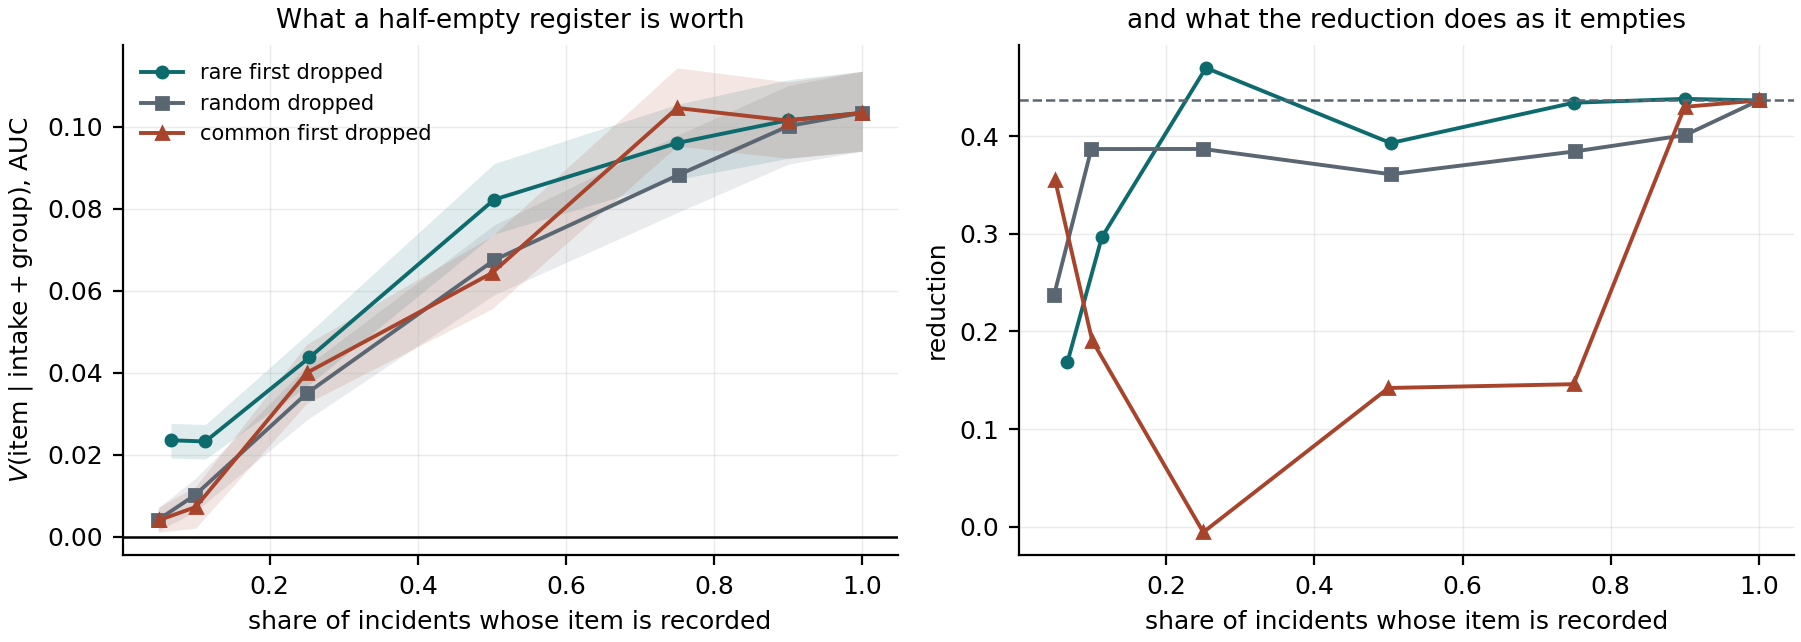
\includegraphics[width=0.86\linewidth]{figK3_population.png}
\caption{What a partially populated register is worth. Left: the item's value
over intake plus the opening group, against the share of incidents whose item
is recorded, under three degradation regimes. Right: the reduction of
Equation~\ref{eq:reduction} on the same axis. The estate is concentrated
enough that $246$ of $2{,}929$ items carry $90\%$ of the incidents, which is
why dropping the tail costs so little.}
\label{fig:population}
\end{figure}

The practical reading is that a buyer who prices a half-populated register
from the random curve will be wrong in whichever direction their estate
actually degrades, and by roughly a factor of three in the reduction. The
usual caveat --- ``our figure is an upper bound because real data is worse''
--- is not supported on this axis either: at full population the measurement
sits at the top of its own curve, so better discovery tooling cannot raise it.

\section{The Four Axes, on Three Organisations}
\label{sec:threelogs}

Everything to this point varies the four choices on one log, and a referee is
entitled to say that ``each choice moves the answer by more than the effect''
is then an $n=1$ claim. The corpus of Section~\ref{sec:corpus} finds three
logs on which the reduction is resolvable: BPI Challenge 2014 (a Dutch bank's
IT operation, HP Service Manager), BPI Challenge 2013 incidents (Volvo IT
Belgium, VINST) and BPI Challenge 2019 (a multinational coatings
manufacturer's procurement process, SAP). Three organisations, three
information systems, two domains. \texttt{r44\_axes\_multilog.py} runs the
whole surface on all three through one code path: a four-rung baseline ladder
giving six ordered nested pairs, four scalar instruments, the $31$-point net
benefit grid, and four register-population levels under two degradation
regimes.

\begin{table}[htbp]
\centering
\caption{The range of the range. For each log, the reduction $R$ at the
reference cell, and the interval $R$ occupies as each choice alone is varied
with the other three held at the reference. The threshold column is
restricted to the grid points where the naive net-benefit increment is at
least a tenth of its maximum, because a ratio whose denominator is positive
but tiny is not a quantity; the unrestricted range is in
\texttt{results/r44\_spread.csv} and is wider.}
\label{tab:threelogs}
\begin{tabular}{lrrrrr}
\toprule
log & $R$ & baseline & metric & operating point & population \\
\midrule
BPIC 2014           & $0.350$ & $[0.010,0.575]$ & $[0.080,0.381]$ & $[-1.728,0.694]$ & $[0.228,0.406]$ \\
BPIC 2013 incidents & $0.378$ & $[0.356,0.823]$ & $[0.147,0.484]$ & $[-0.420,0.872]$ & $[-0.856,0.437]$ \\
BPIC 2019           & $0.471$ & $[0.190,0.844]$ & $[0.471,0.676]$ & $[-7.502,1.570]$ & $[0.462,0.548]$ \\
\bottomrule
\end{tabular}
\end{table}

\paragraph{What replicates, and the rung that has to come out first.}
Across all six nested pairs the baseline choice moves $R$ by $0.565$, $0.467$
and $0.654$ against reference values of $0.350$, $0.378$ and $0.471$ --- more
than $R$ itself on every log. \textbf{That comparison is inflated by a rung no
analyst would build.} The bottom of the ladder is the intercept-only model,
and $V(f \mid \emptyset)$ is large for a reason that has nothing to do with
this paper's argument. Dropping every pair that uses it leaves three real
baselines and three pairs, and the spread falls to $0.346$, $0.347$ and
$0.382$ against the same reference values.

So the honest statement is weaker than the one we first wrote, and it is this:
\textbf{restricted to baselines an analyst would actually build, the baseline
choice moves $R$ by an amount comparable to $R$ --- larger on BPI Challenge
2014 ($0.346$ against $0.350$ is within a hundredth), and smaller on the other
two.} The metric axis moves it by $0.301$, $0.337$ and $0.205$. Both axes
remain between six and ten tenths of the effect being reported, on three
organisations rather than one, and that is what the corpus buys. The claim
that either axis \emph{exceeds} the effect is true of BPI Challenge 2014 and
is not established elsewhere; \texttt{results/r49\_baseline\_spread.csv}
carries both versions and the pairs each is computed over.

\paragraph{What does not.} The population axis does \emph{not} behave the same
way. It moves $R$ by $0.179$ on BPI Challenge 2014, by $0.085$ on BPI
Challenge 2019, and by $1.293$ on BPI Challenge 2013 incidents, where
degrading the register to a quarter populated drives $R$ negative. That is a
fifteen-fold difference across three logs, and the honest reading is that how
much the register's completeness matters is a property of the estate rather
than of the method. Section~\ref{sec:population}'s curve is a measurement on
one estate and the paper does not generalise it.

\paragraph{And the reference cell is a choice too.} The three reference values
$0.350$, $0.378$ and $0.471$ look like a replication. They are three points
picked from three surfaces whose cells span $[0.009, 0.845]$ once the baseline
alone is varied. That agreement is worth exactly as much as the agreement of
any three unstated choices, which is the paper's own argument turned on the
paper's own numbers, and it is why Table~\ref{tab:threelogs} prints the
intervals beside the points rather than the points alone.

\section{The Estimator Against an Answer That Is Known}
\label{sec:sim}

Every number to this point is estimated and none is checked against a truth,
because on a real log there is no truth to check against. A referee who
believes the estimator is biased --- a ratio of two differences of two fitted
AUCs is not an obviously well-behaved thing --- has so far had nothing to read.
This section builds a world where the answer is known by construction and asks
the paper's own estimator for it.

\paragraph{The construction.} Four discrete variables on a finite cell space:
an intake block $b$ with $4$ levels, a free opening field $g$ with $6$, a
high-cost entity $f$ with $40$, and a binary outcome whose log-odds are
$e_b[b] + (1-\rho)\,e_f[f] + \rho\,e_g[g] + c$. The overlap $\rho$ is the share
of the entity's effect on the outcome that the opening field also carries;
$g$ is a many-to-one coarsening of $f$ corrupted at a fixed rate, which is what
a resource stamp and a register look like in a real log. The space is
$960$ cells, so every conditional --- and therefore the Bayes-optimal score
given any feature set, and therefore the population AUC of that score with
ties taking half credit --- is computed by \textbf{exhaustive enumeration}
rather than by sampling. That gives $R^{*}(\rho)$ exactly.

\paragraph{What the truth looks like.} $R^{*}$ rises monotonically with the
overlap, from $0.133$ at $\rho = 0$ --- where $g$ still absorbs something,
because it is a coarsening of $f$ and predicts on its own --- to exactly
$1.000$ at $\rho = 1$, where $V(f \mid B_0 \cup \{g\})$ is zero to machine
precision because $g$ carries everything $f$ has. At $\rho = 0.4$,
$R^{*} = 0.308$; at $\rho = 0.6$, $R^{*} = 0.600$. The estate that produces
the paper's own headline sits between those two, which is worth stating
because it means the measured reduction on BPI Challenge 2014 is what a world
with roughly half the entity's signal in the opening field would produce.

\paragraph{Bias and coverage.} Forty independent replicates per overlap level
at $n = 60{,}000$, each run through the paper's estimator --- one-hot,
logistic, $70/30$ split by row order, paired bootstrap over test rows with one
index set per draw shared by all four models.

\begin{table}[htbp]
\centering
\caption{The estimator against a known answer, $40$ replicates at
$n = 60{,}000$ per row. Coverage is the share of replicates whose paired
bootstrap $95\%$ interval contains $R^{*}$.}
\label{tab:sim}
\begin{tabular}{rrrrrr}
\toprule
overlap $\rho$ & $R^{*}$ & mean $\hat{R}$ & bias & s.d. & coverage \\
\midrule
$0.0$ & $0.1329$ & $0.1290$ & $-0.0039$ & $0.0112$ & $0.900$ \\
$0.2$ & $0.1559$ & $0.1514$ & $-0.0044$ & $0.0096$ & $0.975$ \\
$0.4$ & $0.3078$ & $0.3065$ & $-0.0013$ & $0.0136$ & $0.925$ \\
$0.6$ & $0.6000$ & $0.6008$ & $+0.0008$ & $0.0139$ & $0.975$ \\
$0.8$ & $0.8766$ & $0.8787$ & $+0.0021$ & $0.0094$ & $0.975$ \\
$1.0$ & $1.0000$ & $1.0027$ & $+0.0027$ & $0.0028$ & $0.850$ \\
\bottomrule
\end{tabular}
\end{table}

The largest absolute bias is $0.0044$ --- a third of one standard deviation of
the estimator itself --- and it shrinks with the sample: the mean absolute
bias is $0.0217$ at $n = 5{,}000$ and $0.0025$ at $n = 60{,}000$. Coverage
runs $0.850$ to $0.975$ against a nominal $0.95$, mean $0.933$. \textbf{The
estimator this paper uses is very nearly unbiased for the quantity this paper
reports, and its interval is close to nominal, on a world where the quantity
is known.}

\paragraph{The one place coverage is poor, and why.} At $\rho = 1$ the true
reduction is exactly $1$, which is the boundary of the parameter space: the
estimator's sampling distribution is squeezed against it, $\hat{R}$ sits
$+0.0027$ above on average, and coverage falls to $0.850$. That is the
behaviour any interval has at a boundary and it is reported rather than
smoothed. It matters for reading Section~\ref{sec:failed}, whose measured
reduction against the intake baseline is $99.7\%$: an interval near $1$ should
be read as weaker evidence than one in the middle of the range.

\paragraph{And the surface behaves as the propositions require.} On the same
worlds, varying the four choices moves $R$ away from $R^{*}$ by amounts that
differ by axis and by world: the baseline axis by up to $0.606$, the threshold
axis by up to $4.014$, the metric axis by up to $0.187$ and the population
axis by up to $0.054$. The ordering --- baseline and operating point large,
metric and population smaller --- is the same ordering the three real logs
produce in Table~\ref{tab:threelogs}, on data whose generating process nobody
chose to make agree with them.

\paragraph{What this does and does not establish.} It validates the
\emph{estimator}, not the \emph{estimand}: a world built from a logistic model
and fitted with a logistic model is a friendly world, and the bias reported
here is a lower bound on the bias against a misspecified truth. It is also
entirely era-independent, which answers part --- and only part --- of the
objection that the newest log in the corpus is from $2019$.

\section{The Corpus: Where the Effect Appears, and Where It Does Not}
\label{sec:corpus}

Everything above is one log. This section asks whether the admissibility
effect is a property of process event logs in general or of ITSM data in
particular, under a protocol registered before any of it was run.

\subsection{Pre-registration}
\texttt{PROTOCOL.md}, supplied as supplementary material and committed to the
repository in a commit that adds no result file, fixes in advance: the two
targets, both reported for every log; the rules that assign every attribute to
exactly one of the high-cost entity $f$, the free per-event field $g$, the
intake block $B_0$, a layer, or excluded; six exclusion codes; the estimator,
split, seed and instruments; the log-level discriminators, computed before any
model is fitted; and the outcome that would falsify the claim. Eight
amendments were made after running the role assignment, which reads no
outcome, and before fitting any model; each is recorded in that file with its
reason, and every one is the registered text failing to implement its own
stated intent. The check that they stop there is that after them the generic
rules assign the primary log exactly the roles this paper assigns by hand ---
$f$ the configuration item, $g$ the opening group, $B_0$ the four intake
fields, and the CI type and subtype as layers --- although nothing in the
rules names that log or those fields.

\paragraph{The corpus, and what the rules exclude.}
The registered rules admit $13$ of the $22$ logs that parse and exclude nine by code. The exclusions are a finding rather than an accident and are set out in Appendix~\ref{app:exclusions}: in BPI Challenge 2012 and every BPI Challenge 2020 sub-log \emph{every case is opened by the same actor}, so there is no free opening field and the question this paper asks cannot arise.

\subsection{The result, which is mostly negative}
Nineteen log-target pairs survive the exclusion rules.
Figure~\ref{fig:corpus} shows every one where a reduction exists to be
measured. On $10$ of the $19$ the entity is not resolvably worth anything over
the intake block at all, so there is nothing for a free field to absorb and
$R$ is undefined rather than small. On the remaining nine the reduction's own
interval excludes zero on four, drawn from three logs: the primary log on both
targets, BPI Challenge 2013's incident log on the duration target
($37.8\%$ $[12.8,62.8]$), and BPI Challenge 2019's procurement log on the
duration target ($47.1\%$ $[40.8,53.4]$ on $251{,}734$ traces).

\begin{figure}[t]
\centering
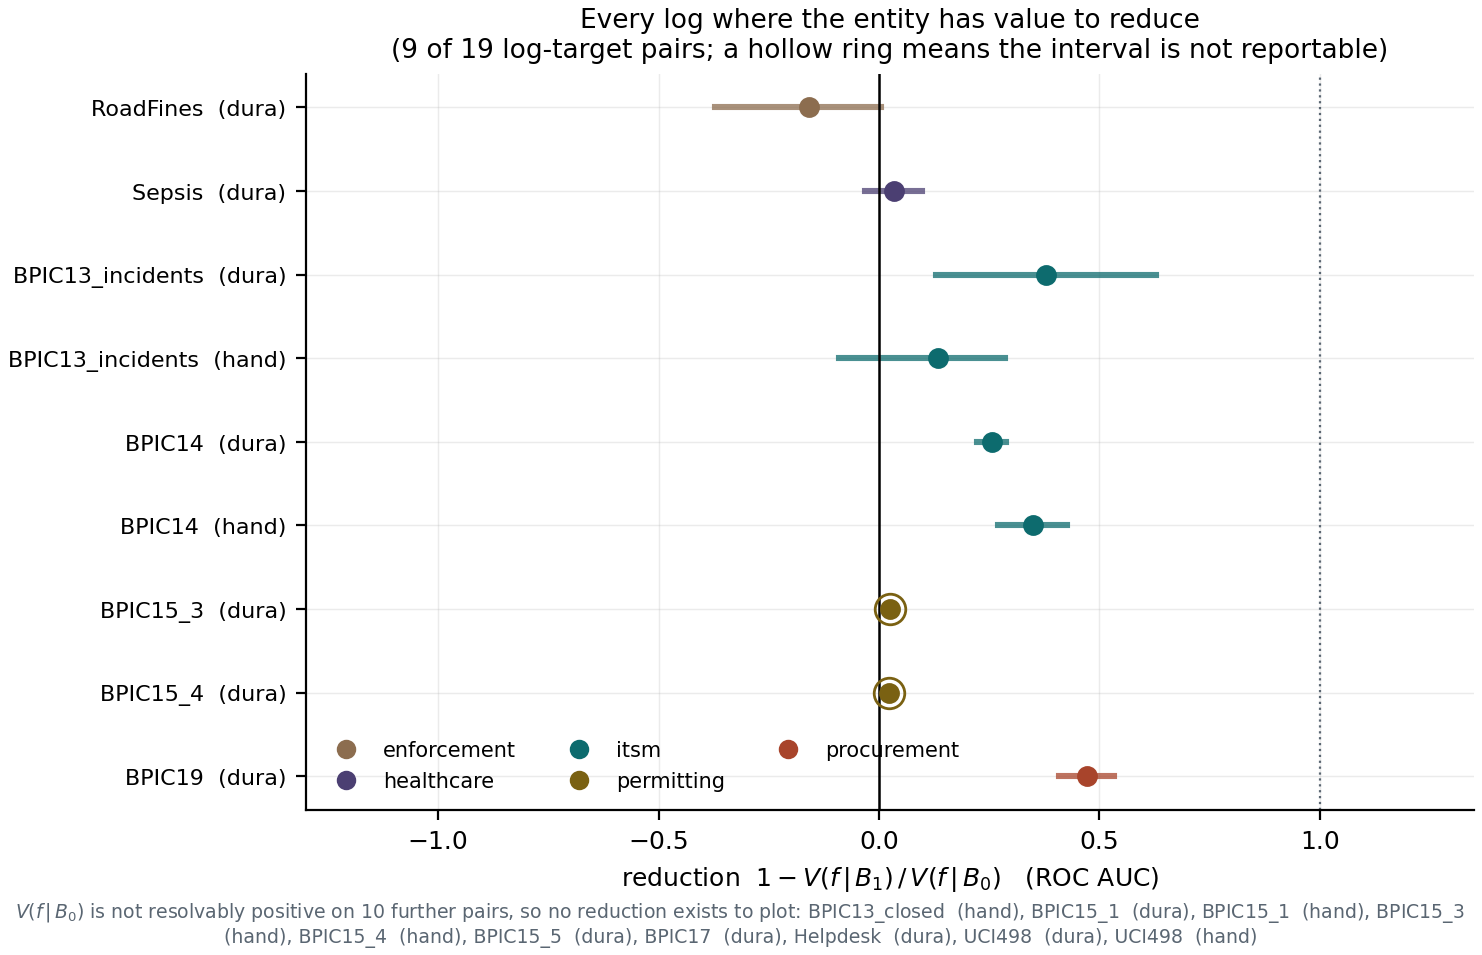
\includegraphics[width=0.86\linewidth]{figK4_corpus.png}
\caption{Every log-target pair where the entity is resolvably worth something
over the intake block, so that a reduction exists. A hollow ring marks a pair
whose reduction has no reportable interval because the denominator is not
positive in every draw.}
\label{fig:corpus}
\end{figure}

Eight of the $13$ admitted logs are outside ITSM, and the reduction is
resolvable on one of them. \texttt{PROTOCOL.md} \S8 states that the claim is
falsified if the effect appears on the two published ITSM logs and not on a
majority of the admitted non-ITSM logs. It is falsified. We report that rather
than reframing the claim to fit, and the paper's scope is bounded accordingly:
what generalises is the \emph{estimand} and the practice of reporting it as a
surface, not the magnitude of any particular reduction.

\paragraph{What ``falsified'' does and does not mean here.}
A referee is entitled to object that we did not fail to find the effect so
much as fail to have a test: on $10$ of the $19$ pairs the reduction has no
denominator, so it could not have been detected had it been there. The
objection is correct and the two statements are separated rather than
conflated. The claim registered in \texttt{PROTOCOL.md} \S8 is falsified
\emph{by its own registered criterion}, which we report because
pre-registration is worth nothing if the verdict is renegotiated once the
answer is known. Beside it: on the nine pairs where a reduction exists to be
measured, four are resolvably positive; on the other ten there was nothing to
measure. A narrower claim --- that where a high-cost entity predicts the
outcome at all, a free opening stamp absorbs a large share of what it is
credited with --- is neither refuted by this corpus nor asserted by it.

\paragraph{Which target carries this.}
Both registered targets are reported for every log, and the four resolvable
results are carried by the \emph{duration} target, which is the standard
outcome in this literature. The handover target is a generalisation of this
paper's own task rather than a standard one, and Section~\ref{sec:corpus}'s
validity check below is why we do not lean on it.

\paragraph{Two things the protocol does not do, stated rather than left to be
found.}
It admits no inter-case features, although Section~\ref{sec:admission} shows
four free creation-time congestion features move the primary log's reduction
from $43.7\%$ to $45.7\%$; that is one log's evidence and the corpus does not
extend it. And its \texttt{NO\_HEADROOM} rule reads the target's prevalence on
the full log, which includes the test half. Recomputing that rule on the
training half only changes \textbf{no} admission decision on any of the $26$
log-target pairs it applies to, so the peek exists in the registered text and
changes nothing in the result.

\paragraph{Two things the corpus does establish.}
Two things survive the negative --- a per-entity historical rate with no model and no attribute that reaches $6.1\%$ to $109.3\%$ of what the fitted model reaches above chance, and a validity check showing the generic target is not this paper's published one. Both are in Appendix~\ref{app:corpusest}.

\subsection{From an explanation to a registered prediction}
\label{sec:prediction}

The paragraph above is an explanation written after seeing the corpus, and an
explanation written after seeing the data is worth very little. This project
had one opportunity to convert it into a prediction and took it.

\paragraph{What was registered, and when.} \texttt{PREDICTION.md} was
committed \emph{before} either held-out log was downloaded, let alone parsed:
at the moment of that commit \texttt{data/normalized/} contained no parquet
for either, \texttt{results/} contained no held-out result, and the script
that downloads them did not exist. Two logs were held out --- BPI Challenge
2011, a Dutch academic hospital, and BPI Challenge 2018, EU agricultural
subsidies --- both recorded in \texttt{PROTOCOL.md} \S2 in the previous round
as considered and not included, for size and parsing cost, and neither ever
opened by this project.

The registered rule: $R$ will be resolvably positive \emph{iff} (i)
$V(f \mid B_0)$ is resolvably positive and (ii) the opening field clears a
threshold fixed numerically from the thirteen logs of Section~\ref{sec:corpus}.
Two forms of (ii) are registered, and the reason is itself a finding.

\paragraph{The form we intended to register fails on its own training data.}
Condition (ii) as first written --- the \emph{normalised entropy} of the
opening field exceeds $H^*$ --- reaches an in-sample balanced accuracy of
$0.600$ on the nine pairs that have a denominator: four true positives, four
false positives, one true negative. Fitted, $H^* = 0.331293$ amounts to
``every log except Sepsis''. The flagship log has the second \emph{lowest}
normalised entropy of the nine, because dividing by $\ln k$ ranks a
seven-valued field spread evenly above a fifty-seven-valued field with a heavy
skew. We report that rather than quietly substituting a rule that works.

\paragraph{The form the data support.} Condition (ii) as
$V(g \mid B_0) > V^* = 0.013302$ --- the opening field's own incremental AUC
over the intake block --- separates all nine training pairs: four true
positives, five true negatives, balanced accuracy $1.000$. It is also what the
mechanism implies, since a field worth nothing over the intake block cannot
absorb anything. \textbf{It was chosen after seeing that the entropy form
failed, and the registration says so.} A rule selected on the training data
can only be tested on data it was not selected on, which is what follows.

\paragraph{The test, and how little it establishes.} BPI Challenge 2011 is
admitted by the registered rules and yields two scored pairs. \textbf{What the
rules picked there is worth stating, because it is not what they were written
for}: the high-cost entity is \texttt{case:Diagnosis}, $102$ distinct values
reused across $11.2$ cases each. A diagnosis is a classification, not a
maintained register that costs money to keep, and \texttt{PROTOCOL.md} \S3.3
admits it because it satisfies a cardinality test and a reuse test, not
because anyone judged it a register. What follows is therefore a prospective
test of the registered \emph{rules} on a log they had never seen, which is
what was registered, and not a test of this paper's question on a hospital.
On both,
$V(f \mid B_0)$ is not resolvably positive --- $-0.0117$
$[-0.0351,+0.0001]$ on duration and $+0.0006$ $[-0.0051,+0.0069]$ on handover
--- so both rules predict ``not resolvable'', and on both the observed
reduction is indeed not resolvable. Two predictions, two correct, zero errors
for each rule. BPI Challenge 2018 is \emph{excluded} on both targets by
registered codes: \texttt{NO\_TEST\_VARIATION} on duration and
\texttt{NO\_HEADROOM} on handover, where the generic handover target has
prevalence $1.0000$ because a seven-valued resource stamp changes at least
once in every one of $43{,}809$ cases --- a mean of $10.14$ distinct values
per case. \textbf{That exclusion is the paper's own mechanism and not an
accident}: $99.9\%$ of those cases open with the literal value
\texttt{0;n/a}, so the opening field carries essentially nothing at intake and
there is no free information for the entity's value to be absorbed by. It is
the same condition as BPI Challenge 2012's and every BPI Challenge 2020
sub-log's, in a form that passes the cardinality rule and fails the target
instead. Excluded pairs are reported with their
code and are not scored; counting an exclusion rule as a correct prediction
would be the cheapest possible way to win this test.

\paragraph{What that is and is not evidence for, said plainly.} Both
registered rules survive: neither erred on a scored pair.
\textbf{But both scored pairs are negatives, so the rules' positive half was
never tested at all}, and the prospective test as executed shows only that the
rules do not fire where the entity is worth nothing --- which condition (i)
alone guarantees. \texttt{PREDICTION.md} \S4 stated before the logs were
opened that at most four pairs could be scored and that the test therefore has
very low power. It had less power than that. The precondition is registered,
it is testable, and it has been tested once on two negatives; a reader who
wants it established needs the next held-out positive, and
\texttt{results/r42\_new\_since.csv} records that as of 2026-08-22 no event
log has been published on 4TU since the cut-off, so this round leaves none
unspent.

\section{A Reporting Standard}
\label{sec:standard}

We propose that a feature-value claim be reported as a surface over the
arguments of Equation~\ref{eq:estimand} rather than as a point, and that the
minimum reportable form is:

\begin{enumerate}
\item \textbf{The baseline ladder.} Every already-recorded field admitted to
$B$, named, with the admissibility criterion stated before it is applied, and
$V$ at each rung. A field the organisation already holds and does not admit is
a decision, and its cost is the difference between two rungs.
\item \textbf{At least one integrating and one operating-point instrument.}
On this data the two families differ by more than the effect. Reporting only
one is reporting one of two answers without saying which question was asked.
\item \textbf{The operating range, not a chosen point.} If the claim is
decision-analytic, the whole curve with intervals, and explicitly the region
where the increment is not resolvable or is negative.
\item \textbf{The register's population, if the feature is a lookup.} With the
degradation regime named, because the regime moves the answer by more than the
level does.
\end{enumerate}

Figure~\ref{fig:surface} is that report for one instrument on this data, and
Figure~\ref{fig:instruments} is the same claim across instruments. Neither
figure contains a number that is not in a result file, and every number in
both is re-derived from those files by the checker described in
Section~\ref{sec:corrections}.

\begin{figure}[t]
\centering
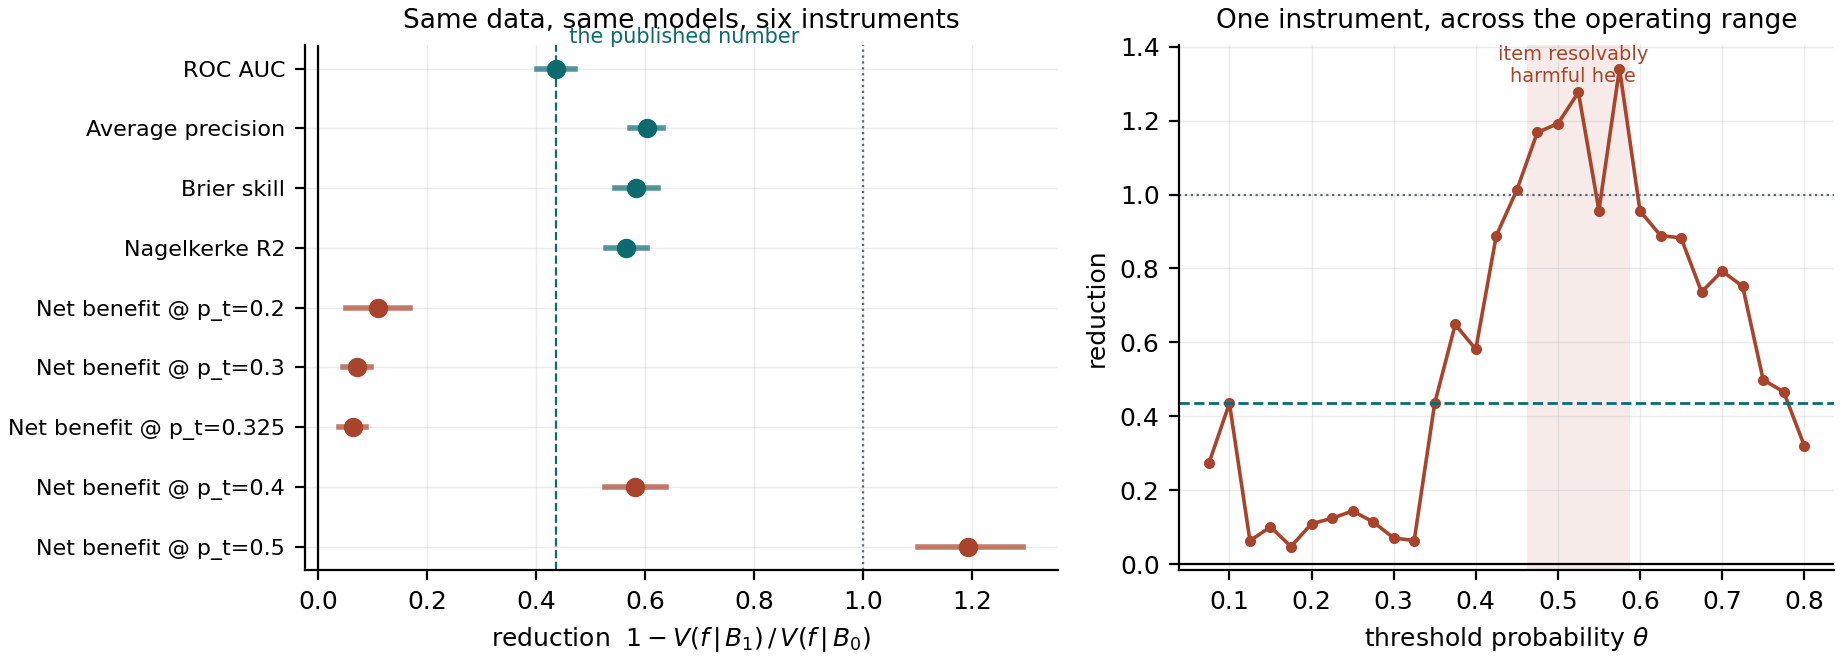
\includegraphics[width=0.86\linewidth]{figK1_instruments.png}
\caption{Left: the reduction under six instruments, paired bootstrap
intervals, the published AUC figure dashed. Right: the same reduction under
one instrument across the operating range. The shaded band is where the item's
increment over a group-aware baseline is resolvably negative.}
\label{fig:instruments}
\end{figure}

\begin{figure}[t]
\centering
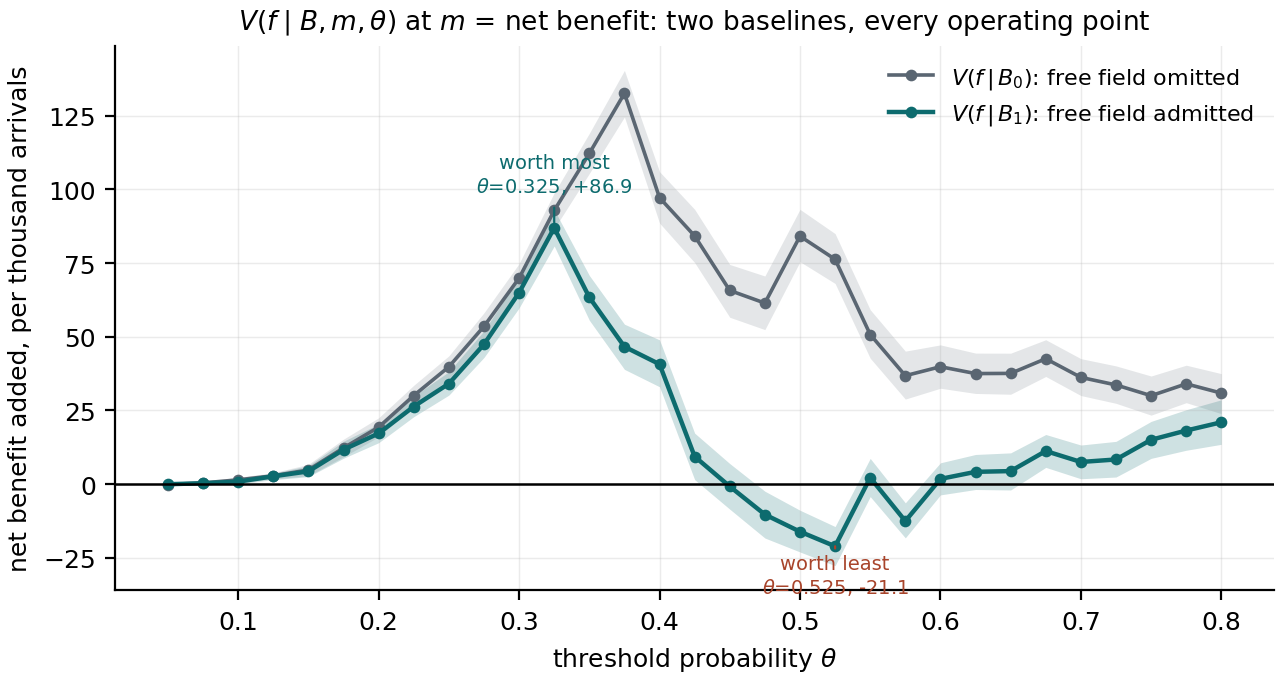
\includegraphics[width=0.86\linewidth]{figK2_surface.png}
\caption{$V(f \mid B, m, \theta)$ at $m$ = net benefit, both baselines, every
operating point, with paired bootstrap bands. A single number for ``what the
item is worth'' is a choice of one $x$-coordinate and one of these two
curves.}
\label{fig:surface}
\end{figure}

\subsection{The standard, as something a reader can run}
\label{sec:tool}

A reporting standard that is a paragraph of prose makes it easier to ignore
than to follow. We ship \texttt{fieldvalue}, a dependency-light Python package
that computes the surface above and \textbf{declines, by design, to emit a
single number}:

\begin{verbatim}
from fieldvalue import surface
s = surface(X, y, feature="ci_name",
            baselines={"intake": INTAKE,
                       "intake+group": INTAKE + ["group"]},
            metrics=["auc", "ap", "brier_skill", "nagelkerke"],
            thresholds=np.arange(0.05, 0.80, 0.025),
            population=[1.0, 0.75, 0.50, 0.25],
            order="opened_at", seed=20260819)
s.report()     # the minimum reportable form, as text
s.to_frame()   # the surface, tidy
s.spread()     # how much each axis moves the answer
s.plot()       # Figure 1
float(s)       # raises SingleNumberRefused, and says why
\end{verbatim}

\noindent There is a command line, \texttt{python -m fieldvalue}, in which
every argument that fixes one of the four axes must be named, because a tool
that defaulted them silently would be the practice this paper is about.

\paragraph{The refusal is the standard, encoded.} \texttt{float(s)} raises
and prints the range the surface actually occupies together with the three
accessors that will answer a properly posed question. A caller who wants one
cell must name it --- \texttt{s.at(baseline=\ldots, metric=\ldots,
threshold=\ldots, population=\ldots)} --- which forces them to say which cell
they are standing in.

\emph{This is not an instruction to put a surface in a business case.} A
business case needs a number, and the standard says what the number is: the
value at one named cell, quoted with its four coordinates, beside the range
the other cells occupy. ``$+0.103$ AUC over an intake-plus-group baseline at
full register population, and between $+0.001$ and $+0.183$ across the
baselines we could defend'' is one sentence, it is what \texttt{s.report()}
prints, and it is the difference between a number and a number whose
provenance a reader can argue with.

\paragraph{An independent code path, and what it found.} The package's metrics
are implemented in numpy from their definitions rather than delegated, so that
re-deriving this paper's headline through it is a real check and not a
tautology; \texttt{fieldvalue}'s test suite asserts agreement with
scikit-learn to $10^{-12}$, so the independence costs no correctness.
\texttt{r46\_tool\_agreement.py} re-derives the surface of
Section~\ref{sec:metric} through the package and compares it against
Section~\ref{sec:metric}'s own pipeline: \textbf{$20$ of $20$ quantities agree,
the largest disagreement being $2.2 \times 10^{-16}$}. What is \emph{not}
independent, and the paper does not pretend it is: scikit-learn's
\texttt{OneHotEncoder} and \texttt{LogisticRegression}, which both paths call,
and the cohort, which both read from the same loader. An error in the
estimator or in the cohort would agree with itself.

The check earned its keep on its first run, and against this paper.
Section~\ref{sec:opp}'s claim that the reduction ``runs $6.3\%$ to $119.2\%$
across the operating range'' named an extremum that was not the extremum: over
the $28$ grid points where the denominator is resolvably positive it runs
$4.7\%$ at $\theta = 0.175$ to $134.1\%$ at $\theta = 0.575$. Every literal in
the old sentence was correct and the relation it asserted was not. It is the
twelfth correction and it is in Section~\ref{sec:corrections}.

\paragraph{Tests, and a worked example on data that is not ours.}
$91$ tests, including the three propositions of Section~\ref{sec:props} as
test cases, so a proposition that stops holding breaks the library and not
only the paper. \texttt{examples/worked\_example.ipynb} runs the whole surface
on UCI Adult, which is not one of this paper's logs, and is the source of
Section~\ref{sec:audit:worked}'s numbers.

\section{The Question We Could Not Answer, Answered}
\label{sec:failed}

The previous version of this paper had a section here titled ``One Thing We
Could Not Establish''. A third field, the knowledge-article reference, sits on
the same \texttt{Open} row, is $100\%$ populated, and costs nothing. Adding it
to the baseline raises AUC to $0.805$ and drives the measured value of item
identity to $-0.003$. Whether that figure belonged in the headline depended on
whether the field is available at creation, and we could not determine it from
the three files we held. That section named the missing evidence: an
interaction detail file shipped in the same public collection, which we had not
obtained.

We obtained it. \texttt{Detail\_Interaction.csv} records $147{,}004$
service-desk interactions.

\paragraph{What it settles.}
$94{,}250$ of those interactions --- $64.1\%$ of the file --- never produce an
incident at all, and $99.7\%$ of those were resolved on the first call. Every
one of them carries a knowledge reference, across $1{,}978$ distinct articles.
A field the incident process assigns cannot be populated on records the
incident process never touches, so the reference is written by the service desk
during the call. Of the incidents that do join an interaction, $92.4\%$ of the
cohort, the interaction opened before the incident in $100.00\%$ of cases with
a median gap of six minutes, and the desk's recorded handling time on it had
elapsed before the incident opened in $98.6\%$.

\paragraph{What it does not settle, and we say so.}
Agreement with the closed record still cannot discriminate. On the $41{,}413$
incidents whose interaction was worked to completion first, the knowledge
reference agrees with its interaction's value on $100.00\%$ and the closure
code --- which is certainly not creation-time --- on $98.97\%$. The reasoning
of the previous version stands: an interaction is itself a closed record. The
subset whose interaction had formally \emph{closed} before the incident opened
contains five incidents, and nothing is concluded from five.

\paragraph{The consequence, which removes our headline.}
Admitting the reference carried by an interaction that was worked to
completion before the incident opened --- populated on $91.1\%$ of the
cohort --- takes the item's measured value from $+0.103$ to $+0.001$
$[-0.002,+0.003]$, a reduction of $99.7\%$ against the intake-only baseline
rather than $43.7\%$. Figure~\ref{fig:knowledge} draws the ladder.

\begin{figure}[t]
\centering
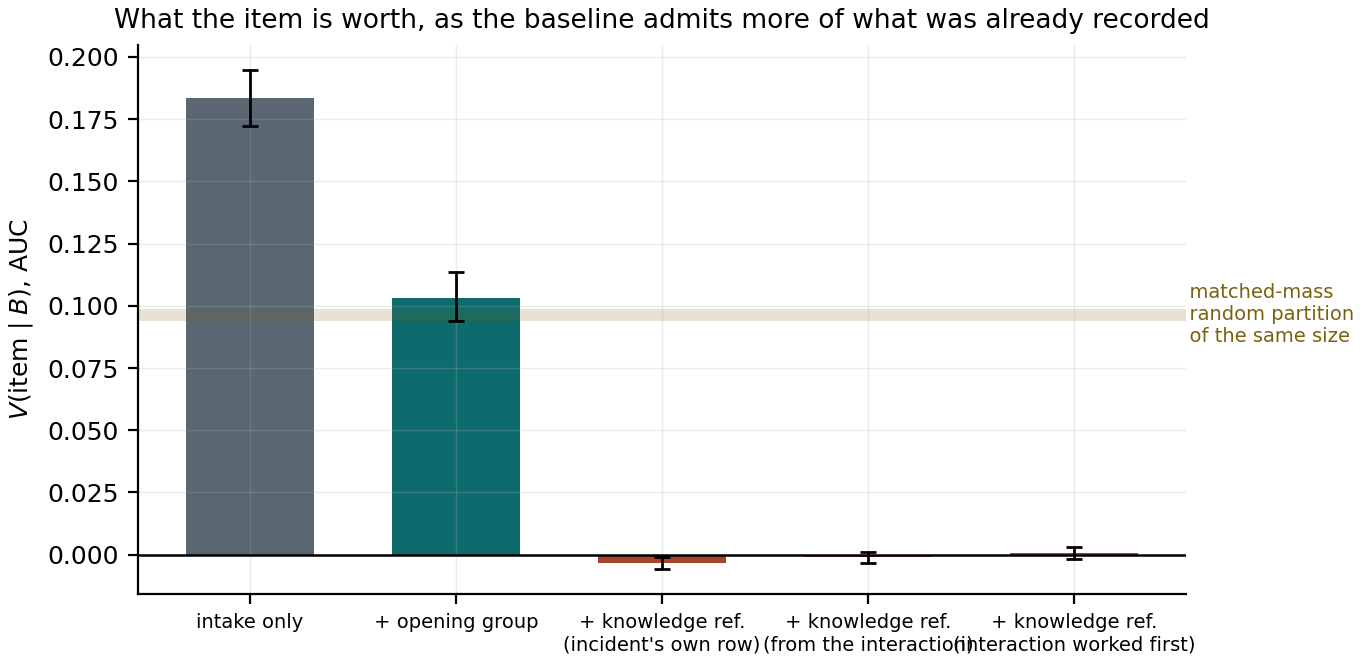
\includegraphics[width=0.86\linewidth]{figK5_knowledge.png}
\caption{What item identity is worth as the baseline admits more of what the
organisation already recorded. The shaded band is the range left by five
matched-mass random partitions of the same cardinality as the knowledge
reference.}
\label{fig:knowledge}
\end{figure}

\paragraph{Three nulls, because a result of that size is not believed on
sight.}
A collapse to zero could be collinearity --- the reference being item identity
relabelled --- or dimensionality, $1{,}700$ extra sparse columns at a fixed
penalty being a burden the item must then overcome, or temporal coherence,
since a knowledge article is used in bursts and a random grouping is not.
\textbf{None survives}, and the three are constructed and measured in
Appendix~\ref{app:nulls}: $78.8\%$ of articles map to exactly one item against
$80.7\%$ for the opening group; five matched-mass random partitions of the
same cardinality reach base AUC at most $0.6479$ where the real field reaches
$0.8041$; and a partition matched on cell size \emph{and} on each cell's
distribution over twenty time strata does not reproduce either number.

\section{Threats to Validity, Each Measured}
\label{sec:threats}

Every threat below has a measurement rather than a paragraph, and each
measurement is somewhere in this paper already. They are collected here so a
reader can see the whole list at once and check that none of them is answered
with an argument.

\paragraph{Construct: the target is not what its name suggests.}
Reassignment is routine handling, not error; it fires on $37.2\%$ of test
incidents. \emph{Measured:} the ladder is reported at stricter target
definitions in Section~\ref{sec:admission}, and the paper says
``reassignment'' rather than ``misrouting'' throughout for that reason.

\paragraph{Construct: the free field is not the routing queue.}
An earlier version asserted it was. \emph{Measured:} three checks in
Section~\ref{sec:data} say otherwise --- $50$ distinct groups on the
\texttt{Open} rows against $218$ on the \texttt{Assignment} rows, one group
holding $67.0\%$ of openings but $18.4\%$ of all activity, and a $15.1\%$
match between the opening group and the first assignment. It is correction
five.

\paragraph{Construct: the corpus does not measure this paper's task.}
The generic handover target is not the primary log's own
\texttt{\# Reassignments} field. \emph{Measured:} prevalence $0.927$ against
$0.411$, agreeing on $46.0\%$ of incidents. Section~\ref{sec:corpus} states
that the corpus measures a generic workflow outcome on twelve further
organisations and not this paper's task, which it would have been easy to
write as though it did.

\paragraph{Internal: the split, and both censoring boundaries.}
A random split on a process log leaks the future, so the split is temporal.
\emph{Measured:} $1{,}150$ left-censored incidents are removed and are
reassigned at $81.2\%$ against $40.0\%$ for those kept; re-measuring on
cohorts truncated up to a month early moves the shrinkage between $42\%$ and
$45\%$, so the right-hand boundary does not drive it.

\paragraph{Internal: the estimator's own knobs.}
\emph{Measured:} the L2 penalty is held fixed across every arm, and tuning it
per arm on an inner split moves the headline reduction from $43.7\%$ to
$43.2\%$; \texttt{Priority} is a deterministic function of
\texttt{(Impact, Urgency)} and dropping it moves intake AUC from $0.562$ to
$0.564$. Two further estimator families are reported in
Section~\ref{sec:admission}.

\paragraph{Conclusion: the estimator might not estimate the estimand.}
A ratio of two differences of two fitted AUCs is not obviously well behaved.
\emph{Measured:} against a world whose true reduction is known by exhaustive
enumeration, the largest absolute bias is $0.0044$ and bootstrap coverage runs
$0.850$ to $0.975$ (Section~\ref{sec:sim}). Where the denominator is not
resolvably positive no ratio is printed at all.

\paragraph{Conclusion: the analysis pipeline might be wrong in one place.}
Every number in this paper came from one pipeline until this round.
\emph{Measured:} an independent implementation re-derives the headline surface
and agrees on $20$ of $20$ quantities to $2.2 \times 10^{-16}$, and found one
error in this paper's prose on its first run (Section~\ref{sec:tool}). What
the check cannot see is stated there: both paths share scikit-learn's
estimator and the same cohort loader.

\paragraph{External: one estate, and then three.}
\emph{Measured:} the whole surface is run on all three logs whose reduction is
resolvable, and the baseline choice moves $R$ by more than $R$ on every one
(Section~\ref{sec:threelogs}). The population axis does \emph{not} replicate,
moving $R$ by $0.085$ on one log and $1.293$ on another, and the paper says
so.

\paragraph{External: the generality claim, registered and falsified.}
\emph{Measured:} $22$ logs, $13$ admitted, resolvable on three;
\texttt{PROTOCOL.md} \S8's falsification condition is met and reported as met.
The precondition that survives was then registered and tested prospectively,
and produced two correct predictions, both negative, which tests only half of
it (Section~\ref{sec:prediction}).

\paragraph{External: the audit reads only what is open access.}
\emph{Measured:} full text was retrieved for $369$ of $600$ sampled papers,
$61.5\%$; the $231$ that were not are recorded with their reason and are not
coded. Nobody can show the loss is uncorrelated with the codes, and
Section~\ref{sec:limits} does not assume it is.

\paragraph{The apparatus itself.}
A verification harness that can be wrong about the paper is a threat to every
number in it. \emph{Measured:} eight holes have been found in this one and
every one was found by its own corruption suite rather than by the harness or
by reading; the suite carries $255$ mutations, each of which changes the
manuscript in one place and requires the checker to notice; the suite's size, the checker's coverage census and the purity
guard that stops the checker modifying its subject are reported in
Section~\ref{sec:corrections} and in \texttt{REPRODUCE.md}.

\section{Limitations}
\label{sec:limits}

\paragraph{Era, decomposed into four measurements.}
The primary log is six months of 2013 and 2014 from one estate, and practice
has moved. ``Practice has moved'' is not one claim, however, and each of its
four usual components has a proxy in data we hold.
\emph{(i)~Discovery auto-populates the estate.} Ours is already $100\%$
populated, so the measurement sits at the top of its own curve and better
tooling cannot raise it; what a modern estate changes is which part of the
register is populated, and Section~\ref{sec:population} measures that.
\emph{(ii)~Incidents arrive pre-stamped.} In 2014, $97.7\%$ of incidents that
came through the service desk already carried the item their originating call
carried. A change that pre-stamps arrivals is a change from $97.7\%$ to at
most $100\%$.
\emph{(iii)~Service mapping rather than item identity.} The service component
--- $272$ values in this cohort --- reaches $+0.078$ over intake plus group
against the item's $+0.103$, so it captures $75.3\%$ of it, and the item's
marginal over it is $+0.023$.
\emph{(iv)~More intake channels, fewer central desks.} This is the largest
sensitivity in the paper. Subsampling the cohort so that the largest opening
group holds between $0\%$ and $95\%$ of it moves the reduction from $95.3\%$
to $6.3\%$: when one desk opens everything the opening group carries almost no
information and absorbs almost nothing, and when opening is distributed it
absorbs nearly all of the item's apparent value. A 2026 organisation with more
channels sits at the end of that sweep where the free field matters
\emph{more}, not less. Two honest qualifications. Subsampling one estate's
opening groups varies the intake mix \emph{within} one organisation, one tool
and one period; it is a sensitivity, not a replication. What supports reading
it as more than that is Section~\ref{sec:corpus}: the logs in the corpus whose
opening field is nearly constant are exactly the ones that show no effect, so
the sweep's prediction is confirmed on data it was not fitted to.

\paragraph{Data quality.}
Section~\ref{sec:population} replaces the caveat this paragraph used to make.
What remains is that we measure population and not \emph{accuracy}: a register
that is fully populated with wrong values is not modelled here, and we have no
way to detect one in a public export.

\paragraph{Free text, and a search rather than a regret.}
Neither of the published logs carries a usable short description, and every
real deployment has one. \citet{kapel2026change} rank two free-text fields
above CI Name for a related target. We therefore searched: every attribute of
every one of the $22$ parsed logs, against a criterion declared in
\texttt{PROTOCOL.md} \S7 before the search ran. Of $596$ attributes, zero
satisfy it. The field a referee will name, UCI 498's \texttt{u\_symptom}, is
$3.4\%$ unique with a mean length of $10.9$ characters: a coded symptom, not a
description. Two amendments were needed to stop the criterion admitting
formatted identifiers, and they are recorded. The threat is real, it is the
most important open question this study leaves, and it cannot be tested on
public process-mining data. We report the search rather than the regret.

\paragraph{Construct and mechanism.}
Reassignment is a proxy for misrouting and also fires on legitimate
escalation; the within-item shuffle preserves item membership but not other
correlates of identity, so it bounds the proxy share rather than isolating
it; and the opening group's distribution drifts between our halves. After
round sixteen's withdrawals, we do not claim a measured direction for the
mechanism.

\paragraph{The corpus measures a different target from the rest of the paper.}
Section~\ref{sec:corpus} applies a generic handover target so that one rule
can run on twenty-two logs. On the primary log that target and the log's own
reassignment count agree on $46.0\%$ of incidents. The corpus therefore bounds
the generality of the \emph{estimand and the practice}, not of this paper's
particular magnitude, and we say so there rather than letting thirteen log
names imply thirteen replications.

\paragraph{What is still outside reach.}
No deployment, no organisational partner and no practitioner validation; a
single author with no institutional affiliation; public benchmark data whose
newest log is from 2019. None of the four is fixable by further analysis and
we would rather state them than have them inferred.

\paragraph{The operational statement is a detection statement.}
Net benefit counts detections against reviews at a stated exchange rate. It
does not say that a detected incident is a corrected one, that a desk given
the warning would route differently, or what a correct routing is worth.
Section~\ref{sec:buys} also reports a region of thresholds in which the item
is worth nothing or less than nothing over the group-aware baseline, and we
have no mechanism for that beyond over-confident predictions from a
high-dimensional model.

\section{Corrections, and the Classes They Fall Into}
\label{sec:corrections}

Twelve errors of our own are reported as results rather than edited away. A
paper whose thesis is that unexamined choices set the answer cannot suppress
its own, and that is the whole of the reason: it is not candour and it is not
a confession, it is the same evidence the rest of the paper is made of, turned
on the paper.

The twelve incidents, each with its cause and the section it changed, are in
Appendix~\ref{app:incidents} and in \texttt{REFEREE-LOG.md}. What is worth the
main text is not the incidents but the \textbf{classes}, because a class is
transferable and an incident is not. Five account for all twelve.

\paragraph{Class 1 --- a null drawn at the wrong level (three instances).} A
control built to bound a mechanism was constructed at row level while the
quantity it bounds lives at item level, so the association it was meant to
destroy was destroyed by construction and the null could only return zero. The
same control, rebuilt at the right level, was then swept only to $800$ cells
while the leg it bounds uses $2{,}929$, and the margin was read at the cell
count that maximised it. A third instance ran the control on one of the two
rungs whose difference it bounds. \textbf{The general form: a null is a claim
about a level, and a null evaluated at a different level from its target is not
a weak test but a vacuous one.} This is the class this project has repeated
most, and the reason it repeats is that a vacuous null returns a comfortable
number rather than an error.

\paragraph{Class 2 --- a quantity printed without an interval (one
instance).} An operational factor was published as a point estimate, on an
unmatched pair of models, in a paper that elsewhere declines to resolve
$+0.0017$ past two decimals. \textbf{The general form: a paper's precision
standard has to apply to its headline, and the headline is exactly where the
pressure not to apply it comes from.}

\paragraph{Class 3 --- an asserted meaning that no measurement supports (four
instances).} A central field was described as the routing queue for several
versions when it is the group that logged the incident; a public dataset was
described as lacking a field it has, on every case, while a script in our own
repository was already reading it; an estimator-free asymmetry turned out to
be an algebraic identity between two entropies sitting one division apart in
the same file; and a factor's sign turned out to be a tie-break inside a
single tied block holding $93.1\%$ of what the baseline nominates.
\textbf{The general form: a sentence about what a number \emph{means} is a
claim, and it needs a measurement of its own. The apparatus that checks values
never looks at it.}

\paragraph{Class 4 --- a relation between correct numbers (three
instances).} An extremum named at the worst of the points we happened to have
tabulated rather than at the extremum; a count of a set reported as the length
of an interval; and, found this round by the independent code path of
Section~\ref{sec:tool}, a range across the operating range that was the range
across five named thresholds. In all three, \textbf{every individual literal
was correct and sitting in the correct place}, and every one passed a checker
that re-derives each literal from a result file. What was wrong was the word
joining them --- \emph{reaching}, \emph{in a contiguous run from},
\emph{across the operating range}. \textbf{The general form: a directional or
quantifying word is a claim with no number of its own, and a verifier built
around literals is structurally unable to see it.} The checker now compares
each named extremum against the extremum and each stated count against the run
length; that closes three instances and not the class, and the corruption
suite carries mutations that break a relation while leaving every value
correct.

\paragraph{Class 5 --- an admission decision left unexamined (one
instance).} The previous version reported that it could not establish when a
field is written, named the file that would settle it, and did not obtain the
file --- which sits in the same public collection as the three it did obtain.
Obtaining it took the headline from $+0.103$ to $+0.001$. \textbf{The general
form: the cost of not looking is invisible, so it is never weighed against the
cost of looking.} This paper's own thesis predicts the failure, which is why
it is reported as a correction and not as progress.

\paragraph{Three further classes, on the apparatus rather than on the paper.}
The verification harness has had eight holes and \emph{every one was found by
the corruption suite, never by the harness and never by reading}. Three of the
classes generalise past this repository. \emph{A consumer placed above its
producers}: a coverage census and a guard lint each consumed a list that later
code appended to, so both silently stopped seeing the checks written below
them; moving the block is not a fix for a hole whose cause is order, and both
are now functions called from one late block, with a lint that reads the
checker's own source and fails if a check is registered after them.
\emph{A harness that can modify its subject}: a check that read the corruption
suite's size by importing it \emph{ran} it, and every corruption reported
caught because the nested checker refused to start; a clean result was
produced by an apparatus that had checked nothing. The checker now records the
manuscript's SHA-256 before it reads anything and asserts it is unchanged
before it reports. \emph{A checker that reads a pipeline's output cannot see a
pipeline that never runs}: one analysis script had not parsed for thirteen
rounds while $936$ checks passed against the files it was supposed to
produce; the reproduction script now parses every script before it starts.

\paragraph{The direction, which is the only summary worth drawing.} Eight of
the twelve flattered the result, one excused the paper's principal limitation,
two would have made the result larger had they been noticed earlier, and one
removed the result altogether. We draw the obvious inference about the
direction in which unchecked assertions travel, and we do not claim the
thirteenth will be different.

\section{Conclusion}

What a recorded field is worth is not a number. It is
$V(f \mid B, m, \theta)$, and on this decision every one of those arguments
moves the answer by more than the effect we set out to report.

Vary the baseline: knowing which configuration item an incident concerns is
worth $+0.183$ AUC against four intake fields, $+0.103$ once one further field
the organisation already records is admitted, and $+0.001$
$[-0.002,+0.003]$ once a second is. Vary the metric on those same scores: the
reduction runs $43.7\%$ to $60.3\%$ over six instruments, and the figure we
previously published is the smallest of them. Vary the operating point: it
runs $4.7\%$ to $134.1\%$, and in a band above the base rate the item is
resolvably harmful. Vary the register's population and the regime by which it
empties: at half population the item is worth $+0.082$ or $+0.064$ depending
on whether the tail or the core is missing. Vary how the organisation takes
work in: across intake mixes the reduction runs $6.3\%$ to $95.3\%$.

None of those variations is a defect in any instrument or an error in any
measurement. Each is correct about the question it asks. The point is that a
single number answers one of those questions without saying which, and that
the person writing the business case is the person choosing.

We are asked what a buyer should conclude, and on the scope this paper can
speak to the answer is plain. On this task, this estate and this target, a
register that costs money to build and maintain adds nothing measurable over
two fields the organisation already records, and a business case built on
$+0.183$ is pricing that register together with both of them. We do not say
that about registers in general; Section~\ref{sec:corpus} is why we cannot,
and Section~\ref{sec:limits} lists what would have to be true for the sentence
to travel.

We tried to make the finding general and it did not go. A pre-registered
protocol over $22$ public logs admits $13$ and finds a resolvable reduction on
three; the registered generality claim is falsified and Section~\ref{sec:corpus}
reports it. What the corpus does establish is the precondition: the effect
needs an entity that predicts the outcome at all, and on most public process
logs there is not one. What we offer in its place is
Section~\ref{sec:standard}: a minimum reportable form for an incremental-value
claim, demonstrated on data where following it removes the paper's own
headline. That is the strongest evidence we can give that it is worth
following.

\section*{Acknowledgements and Reproducibility}
The manuscript was subjected to seventeen rounds of adversarial review, the
later rounds machine-assisted, in which each round was asked to break the
previous version's claims; the corrections in Section~\ref{sec:corrections}
came from that process. The protocol of Section~\ref{sec:corpus} was
registered in the repository before the analyses it governs were run, in a
commit that adds no result file. The author set every research question, adjudicated
every proposed correction against the data, and is responsible for the
content. The datasets are public
\citep{vandongen2014bpic,steeman2013bpic}; code, figures and a checker that
recomputes every quantity here:
\url{https://github.com/sudhirdixit1/cmdb-field-admission}.

\bibliographystyle{elsarticle-harv}
\bibliography{references}


\appendix

\section{The Proposition Constructions}
\label{app:props}

Each construction below is executed by \texttt{scripts/r41\_propositions.py},
which asserts the resulting numbers against the claim and exits non-zero if
any of them stops holding. A referee who distrusts a proof can run it; a
referee who distrusts the code can read the closed forms.

\subsection*{Proposition 1}

Every model's score takes one of two values, so a model is the pair of counts
$(a,b)$: positives and negatives in the high block. With $P$ positives,
$N = \rho P$ negatives, $\alpha = a/P$, $\beta = b/N$ and
$\pi = 1/(1+\rho)$,
\[
  \mathrm{AUC}(\alpha,\beta) - \tfrac12 = \tfrac12(\alpha - \beta),
  \qquad
  \mathrm{AP}(\alpha,\beta) - \pi
    = \alpha\!\left(\frac{\alpha}{\alpha + \beta\rho} - \pi\right).
\]
The first is half Youden's $J$ and follows from the midrank definition of AUC
with ties taking half credit. The second follows from evaluating the
precision--recall steps at the single threshold that separates the two blocks.

Both baselines are the fully tied model $(\alpha,\beta) = (1,1)$, which has
$\mathrm{AUC} = \tfrac12$ and $\mathrm{AP} = \pi$, so $V = m(\text{model}) -
m(\text{baseline})$ under both metrics. Choose the naive leg
$(\alpha_1,\beta_1) = (d, 0)$ and the honest leg $(\alpha_3, \alpha_3 - d)$ for
$\alpha_3 \in [d,1]$. Then $\alpha - \beta = d$ on both legs, the AUC
increments are equal, and
\[
  R_{\mathrm{AUC}} = 0
  \quad\text{exactly},\qquad
  R_{\mathrm{AP}}(\alpha_3)
   = 1 - \frac{g(\alpha_3)}{g(d)},\quad
  g(\alpha) = \alpha\!\left(\frac{\alpha}{\alpha + (\alpha-d)\rho} - \pi\right).
\]
$g$ is continuous and decreasing on $[d,1]$, so $R_{\mathrm{AP}}$ sweeps
$[0,\, 1 - g(1)/g(d)]$, and the upper end tends to $1$ as $\rho$ grows.

\paragraph{Why it must be built in integers.} The first implementation passed
proportions and rounded $a$ and $b$, so $\alpha - \beta$ was only
\emph{approximately} equal between the legs and $R_{\mathrm{AUC}}$ came out at
$4.4\times 10^{-4}$ rather than at zero. A proposition claiming an exact zero
has to be constructed in integers: $\rho$ is an integer and $dP$ and $dN$ are
integers, so for integer $a_3 \in [dP, P]$ the matching $b_3 = a_3\rho - dN$ is
an integer and the equality is exact. $\rho$ is part of the construction and
not a fixed constant: near $\alpha = d$ the AP increment is steep, so at
$\rho = 199$ a single integer step of $a_3$ moves $R$ by $0.038$ and
$r = 0.05$ cannot be reached, while at $\rho = 9$ the steps near zero are
$0.0007$ and the reachable maximum is only $0.818$. The declared family sweeps
seven $(P,\rho)$ pairs, each kept under $1.2$ million rows so that a referee
can run it, and the chosen cell is recorded per target in
\texttt{results/r41\_prop1.csv}.

\subsection*{Proposition 2}

The witness applies $\varphi(p) = p^{0.55}$, strictly increasing on $(0,1)$,
to the scores of one leg of a four-model ladder built on $20{,}000$ synthetic
rows. The rank vectors before and after are asserted identical. Under ROC AUC
and average precision $R$ moves by exactly $0.000000$; under Brier skill,
Nagelkerke $R^2$ and net benefit at $\theta = 0.20$ and $\theta = 0.40$ it
moves by $2.200$, $1.645$, $4.255$ and $2.681$.

\subsection*{Proposition 3}

Eighteen synthetic estates are generated by varying three declared knobs: how
tightly the opening field is coupled to the entity ($0.15$, $0.55$, $0.85$),
how much of the entity's effect on the outcome the opening field carries
($0.15$, $0.50$, $0.80$), and how strong the entity's effect is ($1.2$,
$2.2$). Nothing in the generator is fitted, so it cannot encode the answer.
For each estate the spread of $R$ along each of the four axes is computed with
the other three held at declared defaults. For each ordered pair $(X,Y)$ the
search reports the two estates whose $X$-spreads agree to within $5\%$ of that
axis's observed range and whose $Y$-spreads differ by the most; the pair is
constructible if that difference reaches $25\%$ of the $Y$ axis's range.

Both tests are \emph{relative} to the axis's own range. An earlier version
used a fixed absolute tolerance of $0.02$, which made every pair with
$X = \text{threshold}$ unconstructible for a reason that is about units --- the
metric axis moves $R$ by tenths and the threshold axis by whole multiples ---
and not about the proposition. The full search, including the two pairs that
do not reach the criterion and the gaps they do reach, is in
\texttt{results/r41\_prop3.csv}.

\section{The Twelve Corrections, One by One}
\label{app:incidents}

Each entry names what was wrong, what replaced it, and the section it
changed.  Section~\ref{sec:corrections} groups them into classes; this
appendix is the record, and \texttt{REFEREE-LOG.md} carries the
objection each one answers.

\begin{enumerate}
\item \textbf{A null that could not fail.} The mechanism's floor was
originally drawn by assigning cell labels per \emph{row}, so two incidents
sharing an item landed in different cells and the association was destroyed
by construction. The null could only return zero, and we published a margin
of $89$ points against it (Section~\ref{sec:mechanism}).

\item \textbf{The same null, rebuilt, was still a knob.} Rebuilt at item
level it was swept only to $800$ cells while the leg it bounds uses
$2{,}929$, and the reported margin was taken at the cell count that maximised
it. At matched granularity the margin is $3.5$ points at $z=0.9$ and we now
withdraw it. This is the fifth time a null in this project has been drawn at
the wrong level.

\item \textbf{An asymmetry that was an algebraic identity.} The
estimator-free evidence for the direction of the mechanism was a ratio of two
uncertainty coefficients, which is identically the ratio of two marginal
entropies. It was published for eight rounds with both entropies sitting in
the same results file, one division away.

\item \textbf{A factor printed without an interval.} The capacity-table
factor was first given as a point estimate, on an unmatched pair of models,
in a paper that elsewhere refuses to resolve $+0.0017$ past two decimals.

\item \textbf{A central field whose meaning we asserted.} The opening group
was described as the routing queue for several versions. It is the group that
logged the incident (Section~\ref{sec:data}).

\item \textbf{A claim about a public dataset that our own repository
refuted.} We wrote that the third public ITSM log has no affected-item field.
It has one, populated on every case, and a script in our own repository had
been treating it as such (Section~\ref{sec:secondorg}). This was the sole
support for describing the study as single-organisation of necessity, which
we had presented as a constraint rather than a choice. It was a choice.

\item \textbf{An operational factor whose sign was a tie-break.} Correction
four gave that factor an interval; this one asked what it measured. At a
$5\%$ review capacity $93.1\%$ of what the naive baseline nominates is drawn
from one tied block, and reordering rows inside that block --- which changes
nothing any model knows --- moves the naive arm from $-26$ to $+608$. We
withdraw the factor and rebuild Section~\ref{sec:buys} on net benefit, which
never breaks a tie. The replacement number is $1.07$, not $4.3$
(Section~\ref{sec:withdrawn}).

\item \textbf{A control run on one of the two rungs it bounds.} The
shuffled-item encoder null was run on the group-aware rung only, while the
reduction it is meant to bound is computed from two rungs, and its residual
under boosting is eleven standard errors from zero rather than noise. Run on
both rungs, the correction moves the boosting reduction by $3.4$ percentage
points, and upward (Section~\ref{sec:admission}).

\item \textbf{An extremum that was the worst of the points we had named.} We
wrote that the group-aware increment turns negative, ``reaching $-16.1$
$[-23.0,-8.9]$ per thousand at $p_t=0.50$''. The word \emph{reaching} names an
extremum. The extremum is $-21.1$ $[-27.7,-14.4]$ at $\theta=0.525$, which is
$31\%$ larger; $0.50$ was in the list of five thresholds our own table
happened to name and $0.525$ was not. Every literal in that sentence was
correct and was computed from a file already in the repository
(Section~\ref{sec:dca}).

\item \textbf{A count and a run reported as the same set.} We wrote that the
increment is resolvably positive ``at $20$ points, in a contiguous run from
$0.100$ to $0.425$''. Fourteen are in that run; six sit at $0.675$ and above.
Counting a set and describing an interval are different operations and this
sentence performed one and reported the other (Section~\ref{sec:dca}).

\item \textbf{An open question we left open with the evidence one download
away.} The previous version reported that it could not establish whether the
knowledge-article reference is available at incident creation, named the file
that would settle where the field comes from, and did not obtain it. The file
is in the same public collection as the three we used. Obtaining it shows the
reference is written by the service desk on calls that never become incidents
at all, and admitting it takes our headline from $+0.103$ to $+0.001$
(Section~\ref{sec:failed}). We record this as a correction rather than as
progress because the paper's own thesis is that an unexamined admission
decision sets the answer, and we left ours unexamined for a round.

\item \textbf{A range across the operating range that was a range across five
named points.} We wrote that under net benefit the reduction ``runs $6.3\%$ to
$119.2\%$ across the operating range''. Those are the values at
$\theta = 0.325$ and $\theta = 0.500$, two of the five thresholds our own
table happened to name. Over the $28$ grid points where the denominator is
resolvably positive the reduction runs $4.7\%$ at $\theta = 0.175$ to
$134.1\%$ at $\theta = 0.575$. Every literal was correct and the phrase
\emph{across the operating range} was not, which makes this the third instance
of the class corrections nine and ten belong to. It was found by the
independent code path of Section~\ref{sec:tool}, on that path's first run,
which is the only reason it was found at all: the checker had a check on each
of $6.3$ and $119.2$ and no check on the word \emph{across}.
\end{enumerate}

\section{Which Layer of Configuration Data Pays?}
\label{sec:layer}

The field-admission question of Section~\ref{sec:admission} has a companion
that is more directly a buying decision, and it is where this paper's
novel finding sits: not whether configuration data is worth anything, but at
what resolution, and whether what pays is the configuration \emph{attributes}
at all. Four nested groupings of the same estate are all $100\%$ populated and
free once the item is known. Measured over the intake-plus-group baseline of
$0.644$:

\begin{table}[t]
\centering\small
\begin{tabular}{@{}lrrr@{}}
\toprule
Grouping & levels & AUC & gain \\
\midrule
CI Type (aff)               & $13$    & 0.671 & $+0.027$ \\
CI Subtype (aff)            & $61$    & 0.657 & $+0.013$ \\
Service Component WBS (aff) & $256$   & 0.722 & $+0.078$ \\
CI Name (aff)               & $2{,}554$ & 0.748 & $+0.103$ \\
\midrule
CI Name, marginal over the service component & --- & --- & $+0.023$ \\
\bottomrule
\end{tabular}
\caption{At what resolution configuration data carries its value, over a
baseline that already contains the opening group. Levels are counted in the
training half.}
\label{tab:resolution}
\end{table}

A $256$-way service-component grouping captures three quarters of what
instance-level identity is worth, and instance identity adds $+0.023$ over
it. The classification layers proper --- CI type and subtype --- carry
little, and CI Subtype scores below CI Type despite being finer, which is
what a fixed penalty does to a sparser column. This is the same $+0.023$ that
Section~\ref{sec:mechanism} reports for admitting the service component to
the baseline, seen from the other side: the two are the same quantity, and a
reader who regards an application or service register as something an
organisation has without a configuration-management practice should read the
CMDB's marginal contribution here as that figure.

\paragraph{Why these fields are in the ladder and not in the baseline.}
The obvious question is why CI Type and CI Subtype, being $100\%$ populated
and free, are not simply admitted to the CMDB-free baseline alongside the
opening group. The answer is the second admissibility criterion of
Section~\ref{sec:data} and it needs no model: both are exact functions of
item identity. Neither varies on a single one of the $2{,}929$ items, so both
exist only where the item register exists, and admitting them would be
admitting the CMDB to the CMDB-free baseline. The service component is the
case this argument does not dispose of, and the quantitative gap is
instructive: it varies on $58$ of $2{,}929$ items, carrying $8.7\%$ of
incidents, where the opening group varies on $565$ items carrying $92.5\%$.
The line between the two fields is real and it is a matter of degree, which is
why we report the headline both ways rather than choosing.

\paragraph{The signal is an outcome history keyed on identity.}
A per-item reassignment rate computed on the training half and applied to the
test half as a lookup table --- no model, no other field, no configuration
attribute of any kind --- scores $0.744$, against $0.745$ for item identity
alone under the full estimator and $0.748$ for the paper's complete model. Whatever the CMDB
supplies here, it is not the item's attributes; it is a stable identifier
under which six months of outcomes can be accumulated. The defensible reading
is that maintaining such an identifier across a changing estate --- dedupe,
reconciliation, retirement --- is itself a configuration-management function,
and we think that reading is right. But it is a different claim from ``the
CMDB is worth $+0.103$'', and an organisation that can key its ticket history
on any stable token can have most of this without one.

\begin{figure}[t]
\centering
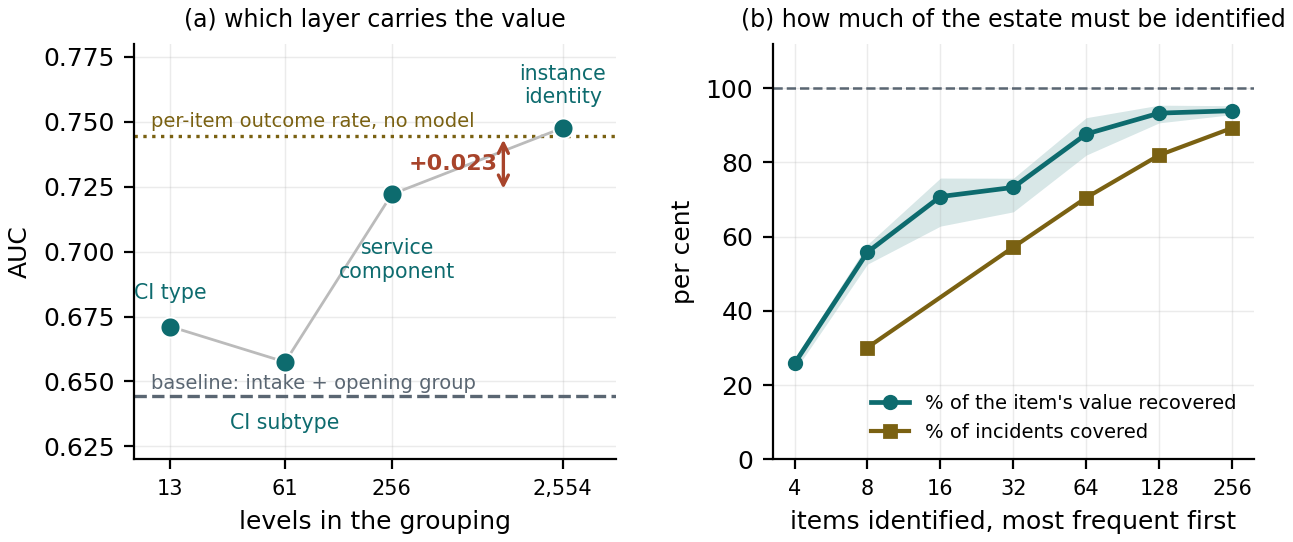
\includegraphics[width=\textwidth]{figJ2_layer.png}
\caption{(a) Which layer carries the value, over a baseline that already
contains the opening group. The dotted line is a per-item outcome rate
applied as a lookup, with no model and no configuration attribute. (b) How
much of the estate must be identified: the share of the item's measured value
recovered by identifying only the $k$ most frequent items, against the share
of incidents those items account for. Band: min--max across five split
points.}
\label{fig:layer}
\end{figure}

\paragraph{Estate concentration.}
Required scope is bounded by a property of the estate needing no model:
the top $8$ items generate $30.2\%$ of training incidents, the top $64$
$70.5\%$, and the top $128$ --- $5.0\%$ of the training vocabulary ---
$82.0\%$, all from a frequency count before funding anything.
Identifying only those items recovers most of the value. Averaged over five
split points, the top $8$ recover $56\%$ of the $+0.103$,
the top $64$ recover $88\%$ and the top $128$ recover $93\%$; across those
splits the three range over $52$--$58\%$, $81$--$93\%$ and $90$--$96\%$.
These are min--max spreads over a design choice, not bootstrap intervals,
and we write them as ranges to keep the distinction. We give the mean and
range rather than one split's curve because a single curve is not monotone at
this resolution: at $k=32$ the across-split spread is $9$ points. The same holds with the group removed from the baseline ---
$89\%$ at $k=64$ --- so this is a property of the estate's concentration, not
of our field-admission decision. Taken with the resolution ladder, the
practical reading is that the marginal AUC of the $2{,}801$ items
outside the top $128$ is small, and that is where the cost of a CMDB
programme lives.

\section{Where the Difference Goes}
\label{sec:mechanism}

The two rows of Table~\ref{tab:headline} differ by $0.080$, which is not
itself informative: for any two
variables, the drop in one's gain when the other joins the baseline equals
the drop in the other's. Read four ways, the item is worth $+0.183$ over
intake and $+0.103$ once the group is present; the group is worth $+0.082$
over intake and $+0.002$ once the item is present.

This section is weaker than the version we published previously, and the
weakening is a finding rather than a concession. Of the four legs that
supported the overlap reading, one has been withdrawn as an algebraic
identity, one no longer resolves once its null is matched properly, and two
survive.

\paragraph{What survives, first.}
Adding the opening group to a model that already knows the
item is worth $+0.0017$ $[+0.0001,+0.0034]$. It clears a matched-dimension
null of $-0.0009 \pm 0.0005$ that no draw reaches, so it is not the cost of
adding columns; but across split points and penalties it ranges $+0.0002$ to
$+0.0072$, so the honest statement is that its unique contribution is
\emph{under $0.01$ AUC and not resolvable more finely}. Because the real
column is nearly constant within an item while the null's is drawn per row,
this null is matched on dimension but not on that collinearity, and a
sceptical reader should treat the interval as the weaker of the two claims.

\paragraph{What survives, second.}
Item identity does not determine the group, but predicts it far better than
chance: a modal-group lookup on item identity reproduces which group logged
the incident on $90.3\%$ of test incidents against $78.6\%$ for always
guessing the largest, while class-balanced accuracy reaches only $34.1\%$.
Item identity resolves the coarse contrast --- central desk or specialist
team --- and much less of the fine one. The two variables share
$1.47$ bits of mutual information.

\paragraph{A margin that was a knob.}
Randomising the group label \emph{within} each item --- which destroys the
label's own identity while preserving what the item implies about it ---
retains $91\%$ of the group's $+0.082$ gain. We previously compared that
against a floor built by randomising within a random partition \emph{of
items} at $49$ cells, matching the opening group's own cardinality, which
retains $42\%$, and reported the $49$-point margin as evidence that item
identity specifically was doing the work.

That comparison is not matched. The real leg partitions on item identity,
which is $2{,}929$ cells; the floor was drawn at $49$. Retention rises
monotonically with the fineness of the partition, so the margin is a
function of a knob that was set to the value maximising it. The stated
ground for stopping the sweep --- that at one cell per item the null becomes
the real thing --- is wrong, because a \emph{random} partition of $n$ items
into $n$ cells is not the identity partition and stays routing-blind. Swept
out to matched granularity the floor retains $87.5\% \pm 3.6\%$ against the
real leg's $91.0\% \pm 1.6\%$: a margin of $3.5$ points at $z=0.9$, against
this project's own resolvability bar of $|z|>3$. We therefore withdraw the
margin. What the sweep shows is that retention is high at fine granularity
whether or not the cells mean anything, which is a fact about granularity and
not about routing.

\begin{figure}[t]
\centering
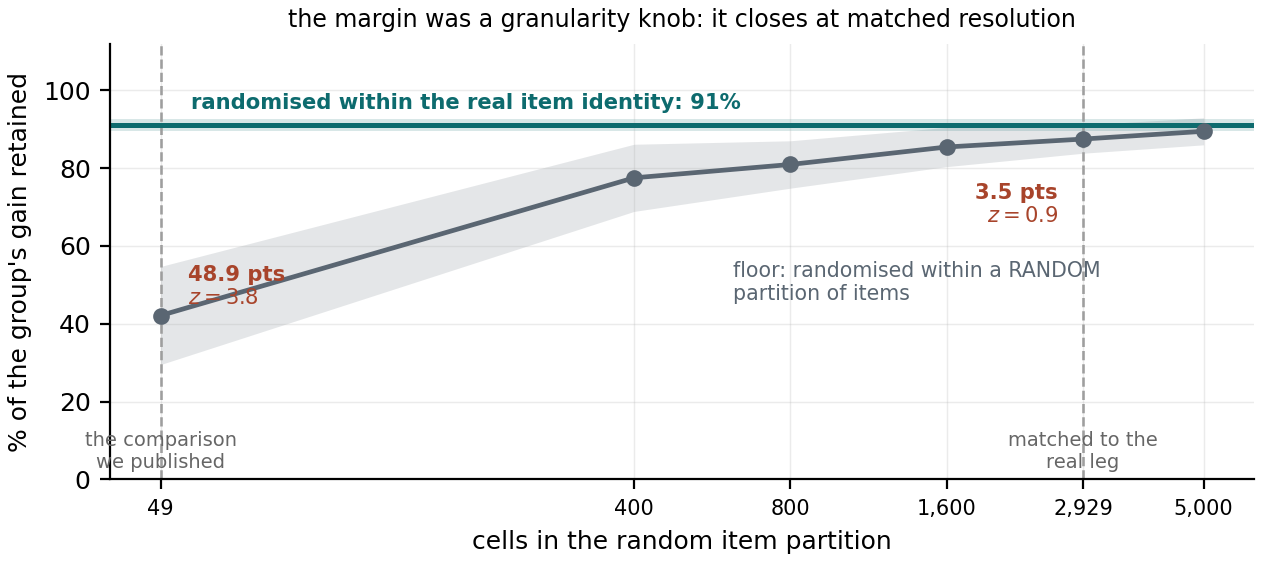
\includegraphics[width=\textwidth]{figJ4_floor.png}
\caption{Randomising the group label within each item, against the same
randomisation within a random partition of items, as a function of how fine
the partition is. The margin we published was measured at $49$ cells; the leg
it bounds partitions on $2{,}929$. It closes as the partition approaches the
granularity of the real leg.}
\label{fig:floor}
\end{figure}

\paragraph{A withdrawn measurement: the asymmetry was an identity.}
We previously reported that, without any estimator, item identity carries
$60.4\%$ of the opening group's information while the group carries $19.6\%$
of the item's, and read the asymmetry as evidence that the mechanism runs
from item to group. The reading is unsupported and the measurement is
circular. The uncertainty coefficient $U(A\mid B) = I(A;B)/H(A)$, and mutual
information is symmetric, so the ratio of the two coefficients is identically
$H(\text{item})/H(\text{group})$ --- a function of two marginal entropies and
of nothing else. On this log that ratio is $3.09$, and the two coefficients,
their shuffled floors, and the floor-corrected excesses we published all
stand in that same ratio to six decimal places. Any two variables whose
entropies stand in that ratio produce those two numbers, whether or not
either determines the other. We withdraw the asymmetry and the directional
claim it supported. The mutual information itself, $1.47$ bits, is a real
measurement and is reported above; its \emph{direction} is not measurable
this way.

\paragraph{The reduction is graded in the field's resolution.}
Coarsening the group and re-running the ladder gives reductions of $27\%$,
$28\%$, $36\%$ and $44\%$ at two, four, eleven and $49$ levels. This is a
consistency check rather than an independent prediction, because at each
resolution the reduction is close to that coarsened field's own gain over
intake --- by the identity above, the same statement as the first
measurement --- and the two coarsest points have overlapping intervals, so
only the trend is claimed. A single binary flag --- central desk or not ---
already recovers $61\%$ of the group's baseline gain and $63\%$ of the
reduction. The field that must be admitted is close to one bit, far cheaper
to reproduce elsewhere than a $49$-way taxonomy.

\paragraph{Is the field really free?}
One objection goes to the heart of the reading. The opening group may be free
only because a human at the desk already knew what the ticket was about ---
in which case it is undocumented configuration knowledge, and a baseline
containing it is not a CMDB-free baseline. A third reading is at least as
likely and we had missed it: the contrast may be an intake-channel
indicator, separating an out-of-hours or overflow or automated route from the
central desk, in which case it is neither independent of the item nor
configuration knowledge held by a person. The one-bit result makes the
question concrete without settling it: the contrast doing most of the work is
the central desk against everything else, and Section~\ref{sec:data} declines
to say what everything else is. The measurement is the same under all three
readings; the moral is not. If the group is independent, a CMDB is worth half
what the naive comparison says. If it is tacit configuration knowledge, our
$+0.103$ is a lower bound and the organisation already holds much of what the
CMDB would tell it, unpaid for. The log cannot identify which is true, so we
choose none of them. What survives either way is that the business case
cannot be written against the intake block alone.

\paragraph{What we do not claim.}
The reverse framing --- that the item column ``stands in for'' the group ---
is not established. We measured it, by randomising items within groups, and
obtained $44\%$ of the item's gain --- but a routing-blind equal-size
partition of items retains \emph{more}, $56\%$, and one whose cell sizes
follow the group's own mass profile retains $25\%$. The leg is floor-dominated and we exclude it. Nor do we claim
a direction of causation: the log records no counterfactual, so whether the
item drives who logs the ticket or both follow a third cause is not
identified here. Our claim is about what an analyst's baseline choice does
to a measured number, which does not depend on which is true.

\paragraph{Two fields we did not admit, and why.}
Our baseline is not a terminus either. Hour of day and day of week are free
and creation-time; adding both moves the item's value from $+0.103$ to
$+0.099$. \texttt{Service Component WBS (aff)} is harder: $100\%$ populated,
free, and admitting it takes the measured value to $+0.023$. We exclude it as
near-deterministic in the item --- only $58$ of $2{,}929$ items carry more
than one value --- so it is configuration data under another name. That
criterion cuts both ways: $2{,}060$ of $2{,}554$ training items also map to a
single opening group, though those items carry just $8.8\%$ of incidents, so
the high-volume ones are the multi-group ones. We know of no principled
threshold that admits the group and excludes the service component. A reader
who draws the line differently should read our headline as $+0.023$ --- which
is the decision this paper is about, and why we report a ladder rather than a
number.

\section{Why the Instruments Disagree}
\label{app:whydisagree}

Three mechanisms are testable and we test all three. Each makes a prediction
that can fail, and the first one did.

\paragraph{Aggregation, which is the largest.}
AUC is $\int \text{TPR}\,d\text{FPR}$, so the increment a feature buys can be
attributed to regions of the operating range without any modelling choice: the
integral is additive over a partition of the FPR axis and the parts sum to the
whole, which we assert rather than assume. We predicted the increment would be
concentrated somewhere the net-benefit grid does not reach. It is not. Over the
$31$-point grid the group-aware model runs at every false-positive rate from
$0.009$ to $0.997$, and the item's advantage is \emph{diffuse}: the largest of
ten equal FPR bands carries $18.2\%$ of it and three bands are needed to reach
half. AUC sums that whole profile; net benefit at one $\theta$ reads one point
of it. The two are not disagreeing about a fact.

\paragraph{Baseline degeneracy, which explains where net benefit is lowest.}
At $\theta = 0.200$, $0.300$ and $0.325$ the intake block acts on every
incident in the test half: as a decision rule it \emph{is} treat-all, and the
group-aware baseline acts on $0.955$ to $0.978$ of them, barely
distinguishable from it.
An increment measured against a rule that does nothing comes out nearly the
same on both rungs, and their ratio near one. Calling a baseline degenerate
when it acts on more than $95\%$ or fewer than $5\%$ of arrivals --- a
threshold we declare before applying it --- the reduction runs $0.047$ to
$0.435$ across the $11$ grid points where both baselines are degenerate and
$0.581$ to $1.168$ across the $5$ where neither is.

\paragraph{Calibration, which is real and provably not the whole story.}
The item-aware model has calibration slope $1.040$ and the intake block
$1.391$. Recalibrating on a held-out tail of the training half moves the
net-benefit reduction by up to $0.253$ where the denominator is safe and the
proper-score reductions by up to $0.014$. It moves the AUC and average
precision reductions by exactly zero, because a monotone rescaling cannot
change a rank statistic --- a prediction that would have failed loudly had the
recalibration not been monotone, and did not.

\paragraph{And a tie convention the two rank statistics do not share.}
The intake block emits $23$ distinct scores for $13{,}637$ incidents.
Average precision's default value equals its \emph{negatives-first} bound, to
machine precision, on all four models, because the precision-recall curve is
evaluated where a tied block has been admitted whole; AUC's default equals a
random tie-break to within $0.0004$. Put both on the only convention a desk
could implement, the reduction is $43.6\%$ under AUC and $71.2\%$ under
average precision. The gap widens rather than closes, which is the outcome we
did not expect and report because we did not.

\section{Why the Capacity Framing Was Withdrawn}
\label{app:capacity}
\label{sec:withdrawn}


The paper already disclosed that the naive baseline cannot rank finely: four
low-cardinality intake fields, one of them the redundant Priority column,
emit only $23$ distinct scores over $13{,}637$ test incidents, so
at $5\%$ capacity just $47$ rows sit strictly above the cut and
the rest come from a tied block of $1{,}944$. It said the factor
was therefore partly about rank resolution rather than information, that the
two had not been separated, and moved on. Separating them destroys the
number.

\begin{table}[t]
\centering\small\setlength{\tabcolsep}{6pt}
\begin{tabular}{@{}lrrr@{}}
\toprule
Tie-breaking policy & naive extra & honest extra & factor \\
\midrule
random --- the only implementable one & $+271$ & $+63$ & $4.3$ \\
oracle: positives first in each tie & $-26$ & $+24$ & --- \\
adversarial: negatives first & $+608$ & $+104$ & $5.8$ \\
\bottomrule
\end{tabular}
\caption{Extra reassignment-bound incidents surfaced at a $5\%$ review
capacity by adding item identity, against a baseline that includes the
opening group (honest) and one that omits it (naive), under three policies
for ordering rows \emph{inside} a tied block. The oracle and adversarial
policies use the outcome and are unavailable to an analyst; together they
bracket what tie-breaking alone can do. Medians of $400$ paired bootstrap
draws over test rows.}
\label{tab:tie}
\end{table}

\paragraph{The naive top-$5\%$ is a draw from a tie.}
Of the $682$ incidents the naive baseline nominates, $635$ --- $93.1\%$ of
the review budget --- come from a single tied block, and that block is
reassigned at $0.534$ against $0.372$ overall. How many of the right
incidents the draw yields is therefore fixed by the block's own base rate and
by nothing the model knows. The $47$ rows the model does rank strictly above
its cut contain $9$ reassignment-bound incidents, a rate below the base rate:
at the top of its own ranking the naive baseline is worse than guessing. The
group-aware baseline is in a different position, with $590$ of $682$ ranked
strictly above the cut and only $92$ drawn from a block of $246$.

\paragraph{The factor's sign is set by the tie-break.}
Table~\ref{tab:tie} prices that. Ordering rows inside the tied block
optimally --- which uses the outcome, so no analyst can --- reverses the sign
of the naive contrast: item identity surfaces $26$ \emph{fewer} incidents
than the intake block alone, not $271$ more. Ordering them adversarially
gives $+608$. Nothing any model knows changes between those three rows. A
quantity whose sign is set by how a coin lands inside a $1{,}944$-row block
is not a measurement of information, and we withdraw it.

A reader may object that the oracle policy favours the coarser arm by
construction: it has the larger block to reorder, so it has the most to gain
from an ordering it cannot obtain. That is the objection restated as the
finding. A contrast whose magnitude is governed by the size of one arm's tie
block, rather than by what either arm knows, is measuring the block. The
random policy is the only implementable one and its value is the one an
analyst would see; but its value is the expected yield of a draw from a
block whose composition is a property of the cohort, not of the ranking,
and the paper should not have read a difference in information off it.

\paragraph{The obvious repair is impossible.}
It is natural to answer the objection by giving the naive baseline a finer
representation, and we tried: cross-fitted target encoding of the intake
block, per field and as a single composite key, on the same machinery used
for the item column in Section~\ref{sec:admission}. It cannot work. The four
intake fields take $23$ distinct combinations, so every row sharing a
combination shares a score under \emph{any} function of those fields, and
combinations unseen in training collapse onto the training prior --- the
composite encoding emits $19$ distinct scores, fewer than the one-hot
model's, not more. The tie block is not an artifact of our estimator. It is
what having four low-cardinality intake fields is.

What survives is narrower and we state it as such: the honest arm's extra
catches are positive under every tie policy, including the oracle
($+24$ $[+9,+40]$), so knowing the affected item does surface more
reassignment-bound incidents at this capacity than the group-aware baseline
does. What does not survive is the ratio, and with it the claim that omitting
the free field overstates the operational gain by more than it overstates the
AUC gain.

\section{The Second Organisation}
\label{app:secondorg}
\label{sec:secondorg}


An earlier version described this study as single-organisation of necessity,
on the ground that of the three public ITSM incident logs in common use, one
records the affected item on every incident, the second on $0.2\%$, and the
third had no such field at all. The third clause was false, and our own
repository contained the evidence: the BPI Challenge 2013 incident log
\citep{steeman2013bpic} from Volvo IT, recorded in VINST, carries a
\texttt{product} attribute with $704$ distinct values, exactly one per trace,
on all $7{,}554$ traces and none missing. It is a coarser identifier than an
instance-level CI name, but it is an affected-item field, and the challenge's
own headline question was ping-pong behaviour between teams --- the same
outcome our primary target measures.

We therefore run the ladder there too. The item analogue is
\texttt{product}; the free field is the \texttt{org:group} on the first
event, of which there are $338$; the intake block is \texttt{impact}, the one
intake-form field the two logs share. The target is at least one change of
\texttt{org:group} along the case, which fires on $50.6\%$ of cases, with a
stricter variant at two or more changes ($27.2\%$). We use the same temporal
$70/30$ split and the same estimator.

One difference cuts against us and we state it rather than let a reader find
it. On BPI Challenge 2014 the opening group matches the incident's first
\texttt{Assignment} group only $15.1\%$ of the time: it is the desk that
logged the ticket, a different object from the routing sequence that defines
the target. On BPI Challenge 2013 the opening group \emph{is} the first term
of the \texttt{org:group} sequence whose variation defines ping-pong. The
coupling is therefore strictly tighter there, the free field is
correspondingly worth more ($+0.188$ against $+0.082$), and the Volvo
reduction should be read as an upper bound rather than as a second draw from
the same distribution.

\begin{figure}[t]
\centering
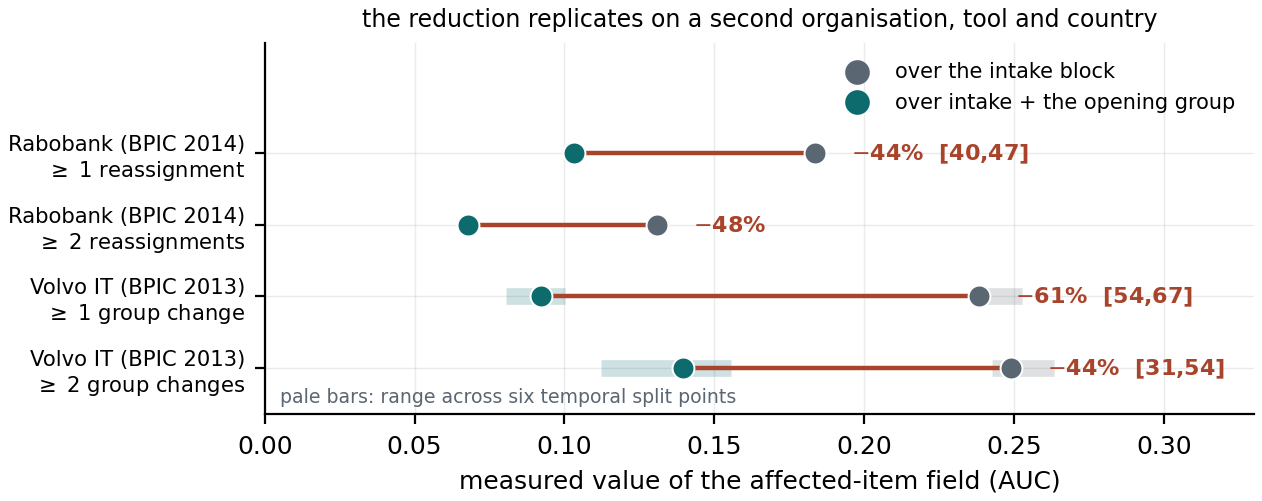
\includegraphics[width=\textwidth]{figJ3_twoorg.png}
\caption{The ladder on both organisations, at two target thresholds each.
Each segment runs from the item's value over the intake block to its value
once the opening group is admitted; the label is the reduction, with its
paired bootstrap interval where one was computed. Pale bars are the min--max
range across six temporal split points, which was computed for the Volvo
rungs only.}
\label{fig:twoorg}
\end{figure}

\section{The Corpus, and What the Rules Exclude}
\label{app:exclusions}

Twenty-four files across seven domains, fetched by DOI with a recorded
SHA-256 for each; $22$ logs parse. The registered rules admit $13$ across six
domains and exclude nine with a code. Two exclusions are worth stating as
findings rather than as bookkeeping. In BPI Challenge 2012 and in all five BPI
Challenge 2020 sub-logs, \emph{every case is opened by the same actor}: the
opening resource stamp has cardinality one, there is no free opening field to
admit, and the question this paper asks cannot arise. In the Hospital Billing
log the only reusable entity, \texttt{diagnosis}, is missing on $65\%$ of first
events and no other attribute reaches the registered cardinality floor.

\section{Two Things the Corpus Does Establish}
\label{app:corpusest}

\paragraph{The condition that governs, and it is measured on the primary log.}
The exclusions are not bookkeeping; they are the answer. BPI Challenge 2015's
five municipalities are the closest thing the public corpus has to a
controlled replication --- one process, five organisations --- four are
admitted, and none shows a resolvable reduction. Their opening resource stamp
has cardinality $7$ to $18$. BPI Challenge 2012 and all five BPI Challenge
2020 sub-logs have cardinality \emph{one}, which is why the protocol excludes
them. A nearly constant opening field cannot absorb anything, and
Section~\ref{sec:limits}'s intake-mix sweep measures precisely that dependence
on the primary log: as the largest opening group's share of arrivals goes from
$0\%$ to $95\%$, the reduction falls from $95.3\%$ to $6.3\%$. A sweep run on
one organisation predicts which logs in the corpus will show the effect and
which will not, and that is the strongest thing the corpus produced.

\paragraph{A precondition, not a moderator.}
We attempted the prediction we set ourselves in advance: regress the
reduction on log properties measurable before any model is fitted --- entity
cardinality, its concentration, the mutual information between $f$ and $g$,
trace length, whether $g$ is a person or a team, and four more. On nine points
with eleven predictors the leave-one-out $R^2$ is $-1.323$ against a
permutation null of $2{,}000$ shuffles at $p = 0.448$: the fit predicts a
held-out reduction worse than its own mean does. We report that and show no
in-sample fit in its place. What the corpus does show is coarser and more
useful: the effect requires an entity that predicts the outcome at all, and on
most public logs it does not.

\paragraph{A generic target is not the published target, and we checked.}
The protocol's handover target counts distinct opening groups in a trace. The
primary log ships its own reassignment count, which is what this paper's other
sections use. They are not the same construction and they do not agree: the
generic target fires on $92.7\%$ of incidents against the published target's
$41.1\%$, and the two agree on $46.0\%$ of them, barely above what
independence between two marginals of that size would give. The tautology
control of \texttt{PROTOCOL.md} \S4.3 splits with them --- under the generic
target the largest opening group has the higher rate, under the published
target the lower. The corpus measures a generic workflow outcome; it does not
measure this paper's task on twelve further organisations, and it would have
been easy to write as though it did.

\section{Three Nulls Behind the Collapse}
\label{app:nulls}

Section~\ref{sec:failed} reports that admitting the knowledge reference takes item identity from $+0.103$ to $+0.001$. A result of that size is not believed on sight, and these are the three nulls that stand behind it.

A collapse to zero could be collinearity --- the reference being item identity
relabelled --- or dimensionality, $1{,}700$ extra sparse columns at fixed
penalty being a burden the item must then overcome, or temporal coherence,
since a knowledge article is used in bursts and a random grouping is not. None
survives.

\emph{Collinearity.} $78.8\%$ of knowledge articles map to exactly one item,
against $80.7\%$ for the opening group, which absorbs less than half of the
item's value rather than all of it. Determinism at that level does not
collapse a marginal.

\emph{Dimensionality.} Five matched-mass random partitions of the same
cardinality --- built by slicing a permutation rather than by
\texttt{searchsorted} on cumulative mass, which is the bug that killed
correction three --- reach base AUC at most $0.6479$ and leave the item worth
$+0.094$ to $+0.099$. The real field reaches $0.8041$ and leaves it worth
$+0.001$.

\emph{Temporal coherence.} Five further partitions matched on cell size
\emph{and} on each cell's distribution over twenty equal-count time strata,
so that every synthetic cell has the same size and the same profile through
time as the real one it copies. They reach base AUC at most $0.6483$ --- the
real field is $0.1558$ above that --- and leave the item worth $+0.092$ to
$+0.101$. We did not build cells from contiguous blocks of the time-ordered
cohort, which would give perfect temporal coherence and would be useless: the
split is temporal, so every test cell would be unseen in training and the null
could not fail. A null that cannot fail is this project's most-repeated defect
and we did not add a sixth.

One thing this ladder does \emph{not} do is condition on a subset. The
knowledge reference enters as a feature column on the unchanged cohort:
incidents whose interaction does not qualify carry an explicit missing token
and stay in the model, the split and the test set, so every rung is measured
on the same $13{,}637$ test incidents.

\paragraph{What this does to the paper.}
Our thesis is that the measured value of a field is set by an admission
decision the analyst makes silently. The strongest available demonstration of
that thesis is that it removes our own headline, and this is that
demonstration. We do not claim the knowledge reference is \emph{proved}
creation-time; we claim the balance of evidence has moved decisively, that a
paper whose headline is contingent on excluding a field must report what
admitting it does, and that $+0.103$ should be read as the value of item
identity \emph{given that one particular free field is admitted and another is
not}. Section~\ref{sec:standard} is the general form of that sentence.

\section{The Decision Curve, in Full}
\label{app:dca}

\label{sec:dca}


\citet{vickers2006dca} supply the instrument the question actually needs.
Fix a threshold probability $p_t$ --- the risk at which a desk judges a
review worth doing --- act on every incident scored at or above it, and
compute
\[
\text{NB}(p_t) \;=\; \frac{\text{TP}}{n} \;-\; \frac{\text{FP}}{n}
\cdot \frac{p_t}{1-p_t}.
\]
The weight $p_t/(1-p_t)$ is the exchange rate the threshold implies: at
$p_t=0.25$ one missed reassignment-bound incident is worth three needless
reviews. Net benefit is in true positives per incident, so we report
$1000 \times \text{NB}$, which reads as reassignment-bound incidents caught
per thousand arrivals net of the reviews spent catching them. It assumes no
capacity, it is defined across the whole range of exchange rates a reader
might hold rather than at one we picked, and --- the point that matters
after Section~\ref{sec:withdrawn} --- a threshold admits or excludes a whole
tied block, so no tie is ever broken.

\paragraph{The scores are probabilities enough for this.}
Net benefit is meaningless for a model whose scores are not calibrated, and a
one-hot logistic model with $2{,}554$ sparse columns at a fixed penalty is
not obviously calibrated. Brier scores run $0.232$ for the intake block,
$0.206$ with the opening group and $0.189$ with the item; calibration slopes
run $1.391$, $1.185$ and $1.040$, so the intake block is the poorly
calibrated arm and the item-aware model is close to ideal. Because a slope
away from one moves net benefit, we repeat the whole analysis on scores
recalibrated on a held-out tail of the training half --- the model refitted
on the first $85\%$ of training, scored on the last $15\%$, and the scaling
applied to test, with no test outcome entering it. No conclusion below
changes.

\begin{figure}[t]
\centering
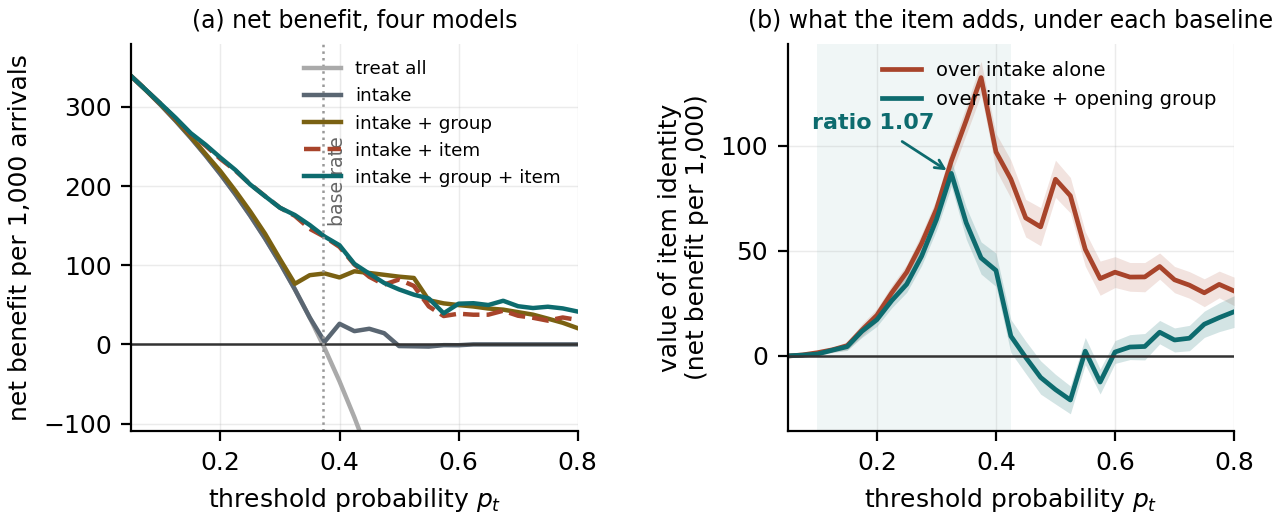
\includegraphics[width=\textwidth]{figJ5_dca.png}
\caption{(a) Net benefit per $1{,}000$ arrivals for the four models and for
treating every arrival, across threshold probabilities. (b) What item
identity adds under each baseline, with $2{,}000$-draw paired bootstrap
bands. The shaded region is where the group-aware increment's interval
excludes zero. The two curves are indistinguishable until the threshold
passes this cohort's base rate.}
\label{fig:dca}
\end{figure}

\begin{table}[t]
\centering\small\setlength{\tabcolsep}{5pt}
\begin{tabular}{@{}lrrr@{}}
\toprule
$p_t$ & over intake + group & over intake alone & ratio \\
\midrule
$0.20$ & $+17.2$ [$14.0,20.4$] & $+19.3$ [$16.0,22.5$] & $1.12$ \\
$0.30$ & $+64.9$ [$59.8,70.2$] & $+69.9$ [$64.7,74.8$] & $1.08$ \\
$0.40$ & $+40.7$ [$33.0,48.9$] & $+97.2$ [$88.6,106.0$] & $2.39$ \\
$0.50$ & $-16.1$ [$-23.0,-8.9$] & $+84.1$ [$75.5,93.2$] & --- \\
$0.60$ & $+1.8$ [$-3.7,7.2$] & $+39.8$ [$32.5,47.2$] & --- \\
\bottomrule
\end{tabular}
\caption{What item identity adds, as net benefit per $1{,}000$ arrivals,
under the two baselines. A ratio is not quoted where the group-aware
increment's interval includes zero or lies below it, because a ratio whose
denominator is crossing zero is not a quantity.}
\label{tab:dca}
\end{table}

\paragraph{Where the item pays, and by how much less than it appears to.}
Over a grid of $31$ thresholds from $0.05$ to $0.80$, the group-aware
increment is positive with its interval excluding zero at $20$ points. Those
$20$ are not one run: $14$ of them form a contiguous block from $0.100$ to
$0.425$, the region either side of this cohort's base rate, and the remaining
$6$ sit at $0.675$ and above, on the far side of the negative band described
below. An earlier version of this sentence said all $20$ lay in the run; every
number in it was correct and the relation asserted between them was not
(Section~\ref{sec:corrections}). The naive increment is positive and resolved
at $29$ of the $31$. At the threshold where item identity is worth most, $p_t=0.325$,
it adds $86.9$ reassignment-bound incidents per thousand arrivals over the
group-aware baseline and $92.8$ over the intake block: omitting the free
field overstates its value there by a factor of $1.07$. This is the number
that replaces the withdrawn $4.3$, and it is smaller than the ratio of
$1.8$ between the same two gains measured as AUC.

\paragraph{And where it does not pay at all.}
Above the contiguous region the increment decays and then turns negative: at
four grid points between $0.475$ and $0.575$ the group-aware increment's
interval lies entirely below zero, and its minimum over the whole grid is
$-21.1$ $[-27.7,-14.4]$ per thousand at $\theta=0.525$. An earlier version
gave the minimum as $-16.1$ $[-23.0,-8.9]$ at $\theta=0.50$, which is the
worst point among the five this paper had chosen to name rather than the worst
point on the grid; the understatement was $31\%$ and it flattered us
(Section~\ref{sec:corrections}). At a one-for-one exchange rate, adding item
identity to a model that already knows the opening group makes the desk worse
off on this task. Locating that band operationally matters, and the direction
is the uncomfortable one: a \emph{higher} threshold means acting on
\emph{fewer} arrivals, so the harmful band is where a capacity-constrained
desk sits, not where an unconstrained one does. Across the four thresholds the
group-aware item model acts on $17\%$ to $37\%$ of arrivals. We have no
mechanism to offer for the sign beyond the obvious one --- a model with
$2{,}554$ item indicators can be confidently wrong where a coarse model
abstains --- and we report it because it is the honest reason the capacity
framing produced the number it did. The earlier version measured the overstatement at the one operating
point where its own group-aware arm had the least to give.

\end{document}
